\documentclass[12pt,a4paper,]{book}
\def\ifdoblecara{} %% set to true
\def\ifprincipal{} %% set to true
\let\ifprincipal\undefined %% set to false
\def\ifcitapandoc{} %% set to true
\let\ifcitapandoc\undefined %% set to false
\usepackage{lmodern}
\usepackage{amssymb,amsmath}
\usepackage{ifxetex,ifluatex}
%\usepackage{fixltx2e} % provides \textsubscript %PLLC
\ifnum 0\ifxetex 1\fi\ifluatex 1\fi=0 % if pdftex
  \usepackage[T1]{fontenc}
  \usepackage[utf8]{inputenc}
\else % if luatex or xelatex
  \ifxetex
    \usepackage{mathspec}
  \else
    \usepackage{fontspec}
  \fi
  \defaultfontfeatures{Ligatures=TeX,Scale=MatchLowercase}
\fi
% use upquote if available, for straight quotes in verbatim environments
\IfFileExists{upquote.sty}{\usepackage{upquote}}{}
% use microtype if available
\IfFileExists{microtype.sty}{%
\usepackage{microtype}
\UseMicrotypeSet[protrusion]{basicmath} % disable protrusion for tt fonts
}{}
\usepackage[margin = 2.5cm]{geometry}
\usepackage{hyperref}
\hypersetup{unicode=true,
            pdfauthor={Francisco José Lozano Ruiz},
              pdfborder={0 0 0},
              breaklinks=true}
\urlstyle{same}  % don't use monospace font for urls
\usepackage{natbib}
\bibliographystyle{plainnat}
\usepackage[usenames,dvipsnames]{xcolor}  %new PLLC
\usepackage{color}
\usepackage{fancyvrb}
\newcommand{\VerbBar}{|}
\newcommand{\VERB}{\Verb[commandchars=\\\{\}]}
\DefineVerbatimEnvironment{Highlighting}{Verbatim}{commandchars=\\\{\}}
% Add ',fontsize=\small' for more characters per line
\usepackage{framed}
\definecolor{shadecolor}{RGB}{248,248,248}
\newenvironment{Shaded}{\begin{snugshade}}{\end{snugshade}}
\newcommand{\AlertTok}[1]{\textcolor[rgb]{0.94,0.16,0.16}{#1}}
\newcommand{\AnnotationTok}[1]{\textcolor[rgb]{0.56,0.35,0.01}{\textbf{\textit{#1}}}}
\newcommand{\AttributeTok}[1]{\textcolor[rgb]{0.13,0.29,0.53}{#1}}
\newcommand{\BaseNTok}[1]{\textcolor[rgb]{0.00,0.00,0.81}{#1}}
\newcommand{\BuiltInTok}[1]{#1}
\newcommand{\CharTok}[1]{\textcolor[rgb]{0.31,0.60,0.02}{#1}}
\newcommand{\CommentTok}[1]{\textcolor[rgb]{0.56,0.35,0.01}{\textit{#1}}}
\newcommand{\CommentVarTok}[1]{\textcolor[rgb]{0.56,0.35,0.01}{\textbf{\textit{#1}}}}
\newcommand{\ConstantTok}[1]{\textcolor[rgb]{0.56,0.35,0.01}{#1}}
\newcommand{\ControlFlowTok}[1]{\textcolor[rgb]{0.13,0.29,0.53}{\textbf{#1}}}
\newcommand{\DataTypeTok}[1]{\textcolor[rgb]{0.13,0.29,0.53}{#1}}
\newcommand{\DecValTok}[1]{\textcolor[rgb]{0.00,0.00,0.81}{#1}}
\newcommand{\DocumentationTok}[1]{\textcolor[rgb]{0.56,0.35,0.01}{\textbf{\textit{#1}}}}
\newcommand{\ErrorTok}[1]{\textcolor[rgb]{0.64,0.00,0.00}{\textbf{#1}}}
\newcommand{\ExtensionTok}[1]{#1}
\newcommand{\FloatTok}[1]{\textcolor[rgb]{0.00,0.00,0.81}{#1}}
\newcommand{\FunctionTok}[1]{\textcolor[rgb]{0.13,0.29,0.53}{\textbf{#1}}}
\newcommand{\ImportTok}[1]{#1}
\newcommand{\InformationTok}[1]{\textcolor[rgb]{0.56,0.35,0.01}{\textbf{\textit{#1}}}}
\newcommand{\KeywordTok}[1]{\textcolor[rgb]{0.13,0.29,0.53}{\textbf{#1}}}
\newcommand{\NormalTok}[1]{#1}
\newcommand{\OperatorTok}[1]{\textcolor[rgb]{0.81,0.36,0.00}{\textbf{#1}}}
\newcommand{\OtherTok}[1]{\textcolor[rgb]{0.56,0.35,0.01}{#1}}
\newcommand{\PreprocessorTok}[1]{\textcolor[rgb]{0.56,0.35,0.01}{\textit{#1}}}
\newcommand{\RegionMarkerTok}[1]{#1}
\newcommand{\SpecialCharTok}[1]{\textcolor[rgb]{0.81,0.36,0.00}{\textbf{#1}}}
\newcommand{\SpecialStringTok}[1]{\textcolor[rgb]{0.31,0.60,0.02}{#1}}
\newcommand{\StringTok}[1]{\textcolor[rgb]{0.31,0.60,0.02}{#1}}
\newcommand{\VariableTok}[1]{\textcolor[rgb]{0.00,0.00,0.00}{#1}}
\newcommand{\VerbatimStringTok}[1]{\textcolor[rgb]{0.31,0.60,0.02}{#1}}
\newcommand{\WarningTok}[1]{\textcolor[rgb]{0.56,0.35,0.01}{\textbf{\textit{#1}}}}
\IfFileExists{parskip.sty}{%
\usepackage{parskip}
}{% else
\setlength{\parindent}{0pt}
\setlength{\parskip}{6pt plus 2pt minus 1pt}
}
\setlength{\emergencystretch}{3em}  % prevent overfull lines
\providecommand{\tightlist}{%
  \setlength{\itemsep}{0pt}\setlength{\parskip}{0pt}}
\setcounter{secnumdepth}{5}
% Redefines (sub)paragraphs to behave more like sections
\ifx\paragraph\undefined\else
\let\oldparagraph\paragraph
\renewcommand{\paragraph}[1]{\oldparagraph{#1}\mbox{}}
\fi
\ifx\subparagraph\undefined\else
\let\oldsubparagraph\subparagraph
\renewcommand{\subparagraph}[1]{\oldsubparagraph{#1}\mbox{}}
\fi

%%% Use protect on footnotes to avoid problems with footnotes in titles
\let\rmarkdownfootnote\footnote%
\def\footnote{\protect\rmarkdownfootnote}


  \title{}
    \author{Francisco José Lozano Ruiz}
      \date{27/10/2017}


%%%%%%% inicio: latex_preambulo.tex PLLC

%% UTILIZA CODIFICACIÓN UTF-8
%% MODIFICARLO CONVENIENTEMENTE PARA USARLO CON OTRAS CODIFICACIONES


%\usepackage[spanish,es-nodecimaldot,es-noshorthands]{babel}
\usepackage[spanish,es-nodecimaldot,es-noshorthands,es-tabla]{babel}
% Ver: es-tabla (en: https://osl.ugr.es/CTAN/macros/latex/contrib/babel-contrib/spanish/spanish.pdf)
% es-tabla (en: https://tex.stackexchange.com/questions/80443/change-the-word-table-in-table-captions)
\usepackage{float}
\usepackage{placeins}
\usepackage{fancyhdr}
% Solucion: ! LaTeX Error: Command \counterwithout already defined.
% https://tex.stackexchange.com/questions/425600/latex-error-command-counterwithout-already-defined
\let\counterwithout\relax
\let\counterwithin\relax
\usepackage{chngcntr}
%\usepackage{microtype}  %antes en template PLLC
\usepackage[utf8]{inputenc}
\usepackage[T1]{fontenc} % Usa codificación 8-bit que tiene 256 glyphs

%\usepackage[dvipsnames]{xcolor}
%\usepackage[usenames,dvipsnames]{xcolor}  %new
\usepackage{pdfpages}
%\usepackage{natbib}




% Para portada: latex_paginatitulo_mod_ST02.tex (inicio)
\usepackage{tikz}
\usepackage{epigraph}
\renewcommand\epigraphflush{flushright}
\renewcommand\epigraphsize{\normalsize}
\setlength\epigraphwidth{0.7\textwidth}

\definecolor{titlepagecolor}{cmyk}{1,.60,0,.40}

%\DeclareFixedFont{\titlefont}{T1}{ppl}{b}{it}{0.5in}

% \makeatletter
% \def\printauthor{%
%     {\large \@author}}
% \makeatother
% \author{%
%     Author 1 name \\
%     Department name \\
%     \texttt{email1@example.com}\vspace{20pt} \\
%     Author 2 name \\
%     Department name \\
%     \texttt{email2@example.com}
%     }

% The following code is borrowed from: https://tex.stackexchange.com/a/86310/10898

\newcommand\titlepagedecoration{%
\begin{tikzpicture}[remember picture,overlay,shorten >= -10pt]

\coordinate (aux1) at ([yshift=-15pt]current page.north east);
\coordinate (aux2) at ([yshift=-410pt]current page.north east);
\coordinate (aux3) at ([xshift=-4.5cm]current page.north east);
\coordinate (aux4) at ([yshift=-150pt]current page.north east);

\begin{scope}[titlepagecolor!40,line width=12pt,rounded corners=12pt]
\draw
  (aux1) -- coordinate (a)
  ++(225:5) --
  ++(-45:5.1) coordinate (b);
\draw[shorten <= -10pt]
  (aux3) --
  (a) --
  (aux1);
\draw[opacity=0.6,titlepagecolor,shorten <= -10pt]
  (b) --
  ++(225:2.2) --
  ++(-45:2.2);
\end{scope}
\draw[titlepagecolor,line width=8pt,rounded corners=8pt,shorten <= -10pt]
  (aux4) --
  ++(225:0.8) --
  ++(-45:0.8);
\begin{scope}[titlepagecolor!70,line width=6pt,rounded corners=8pt]
\draw[shorten <= -10pt]
  (aux2) --
  ++(225:3) coordinate[pos=0.45] (c) --
  ++(-45:3.1);
\draw
  (aux2) --
  (c) --
  ++(135:2.5) --
  ++(45:2.5) --
  ++(-45:2.5) coordinate[pos=0.3] (d);   
\draw 
  (d) -- +(45:1);
\end{scope}
\end{tikzpicture}%
}

% Para portada: latex_paginatitulo_mod_ST02.tex (fin)

% Para portada: latex_paginatitulo_mod_OV01.tex (inicio)
\usepackage{cpimod}
% Para portada: latex_paginatitulo_mod_OV01.tex (fin)

% Para portada: latex_paginatitulo_mod_OV03.tex (inicio)
\usepackage{KTHEEtitlepage}
% Para portada: latex_paginatitulo_mod_OV03.tex (fin)

\renewcommand{\contentsname}{Índice}
\renewcommand{\listfigurename}{Índice de figuras}
\renewcommand{\listtablename}{Índice de tablas}
\newcommand{\bcols}{}
\newcommand{\ecols}{}
\newcommand{\bcol}[1]{\begin{minipage}{#1\linewidth}}
\newcommand{\ecol}{\end{minipage}}
\newcommand{\balertblock}[1]{\begin{alertblock}{#1}}
\newcommand{\ealertblock}{\end{alertblock}}
\newcommand{\bitemize}{\begin{itemize}}
\newcommand{\eitemize}{\end{itemize}}
\newcommand{\benumerate}{\begin{enumerate}}
\newcommand{\eenumerate}{\end{enumerate}}
\newcommand{\saltopagina}{\newpage}
\newcommand{\bcenter}{\begin{center}}
\newcommand{\ecenter}{\end{center}}
\newcommand{\beproof}{\begin{proof}} %new
\newcommand{\eeproof}{\end{proof}} %new
%De: https://texblog.org/2007/11/07/headerfooter-in-latex-with-fancyhdr/
% \fancyhead
% E: Even page
% O: Odd page
% L: Left field
% C: Center field
% R: Right field
% H: Header
% F: Footer
%\fancyhead[CO,CE]{Resultados}

%OPCION 1
% \fancyhead[LE,RO]{\slshape \rightmark}
% \fancyhead[LO,RE]{\slshape \leftmark}
% \fancyfoot[C]{\thepage}
% \renewcommand{\headrulewidth}{0.4pt}
% \renewcommand{\footrulewidth}{0pt}

%OPCION 2
% \fancyhead[LE,RO]{\slshape \rightmark}
% \fancyfoot[LO,RE]{\slshape \leftmark}
% \fancyfoot[LE,RO]{\thepage}
% \renewcommand{\headrulewidth}{0.4pt}
% \renewcommand{\footrulewidth}{0.4pt}
%%%%%%%%%%
\usepackage{calc,amsfonts}
% Elimina la cabecera de páginas impares vacías al finalizar los capítulos
\usepackage{emptypage}
\makeatletter

\definecolor{ocre}{RGB}{25,25,243} % Define el color naranja usado para resaltar algunas salidas

%\usepackage{calc} 

\usepackage{lipsum}

%\usepackage{tikz} % Requerido para dibujar formas personalizadas

%\usepackage{amsmath,amsthm,amssymb,amsfonts}
\usepackage{amsthm}


% Boxed/framed environments
\newtheoremstyle{ocrenumbox}% % Theorem style name
{0pt}% Space above
{0pt}% Space below
{\normalfont}% % Body font
{}% Indent amount
{\small\bf\sffamily\color{ocre}}% % Theorem head font
{\;}% Punctuation after theorem head
{0.25em}% Space after theorem head
{\small\sffamily\color{ocre}\thmname{#1}\nobreakspace\thmnumber{\@ifnotempty{#1}{}\@upn{#2}}% Theorem text (e.g. Theorem 2.1)
\thmnote{\nobreakspace\the\thm@notefont\sffamily\bfseries\color{black}---\nobreakspace#3.}} % Optional theorem note
\renewcommand{\qedsymbol}{$\blacksquare$}% Optional qed square

\newtheoremstyle{blacknumex}% Theorem style name
{5pt}% Space above
{5pt}% Space below
{\normalfont}% Body font
{} % Indent amount
{\small\bf\sffamily}% Theorem head font
{\;}% Punctuation after theorem head
{0.25em}% Space after theorem head
{\small\sffamily{\tiny\ensuremath{\blacksquare}}\nobreakspace\thmname{#1}\nobreakspace\thmnumber{\@ifnotempty{#1}{}\@upn{#2}}% Theorem text (e.g. Theorem 2.1)
\thmnote{\nobreakspace\the\thm@notefont\sffamily\bfseries---\nobreakspace#3.}}% Optional theorem note

\newtheoremstyle{blacknumbox} % Theorem style name
{0pt}% Space above
{0pt}% Space below
{\normalfont}% Body font
{}% Indent amount
{\small\bf\sffamily}% Theorem head font
{\;}% Punctuation after theorem head
{0.25em}% Space after theorem head
{\small\sffamily\thmname{#1}\nobreakspace\thmnumber{\@ifnotempty{#1}{}\@upn{#2}}% Theorem text (e.g. Theorem 2.1)
\thmnote{\nobreakspace\the\thm@notefont\sffamily\bfseries---\nobreakspace#3.}}% Optional theorem note

% Non-boxed/non-framed environments
\newtheoremstyle{ocrenum}% % Theorem style name
{5pt}% Space above
{5pt}% Space below
{\normalfont}% % Body font
{}% Indent amount
{\small\bf\sffamily\color{ocre}}% % Theorem head font
{\;}% Punctuation after theorem head
{0.25em}% Space after theorem head
{\small\sffamily\color{ocre}\thmname{#1}\nobreakspace\thmnumber{\@ifnotempty{#1}{}\@upn{#2}}% Theorem text (e.g. Theorem 2.1)
\thmnote{\nobreakspace\the\thm@notefont\sffamily\bfseries\color{black}---\nobreakspace#3.}} % Optional theorem note
\renewcommand{\qedsymbol}{$\blacksquare$}% Optional qed square
\makeatother



% Define el estilo texto theorem para cada tipo definido anteriormente
\newcounter{dummy} 
\numberwithin{dummy}{section}
\theoremstyle{ocrenumbox}
\newtheorem{theoremeT}[dummy]{Teorema}  % (Pedro: Theorem)
\newtheorem{problem}{Problema}[chapter]  % (Pedro: Problem)
\newtheorem{exerciseT}{Ejercicio}[chapter] % (Pedro: Exercise)
\theoremstyle{blacknumex}
\newtheorem{exampleT}{Ejemplo}[chapter] % (Pedro: Example)
\theoremstyle{blacknumbox}
\newtheorem{vocabulary}{Vocabulario}[chapter]  % (Pedro: Vocabulary)
\newtheorem{definitionT}{Definición}[section]  % (Pedro: Definition)
\newtheorem{corollaryT}[dummy]{Corolario}  % (Pedro: Corollary)
\theoremstyle{ocrenum}
\newtheorem{proposition}[dummy]{Proposición} % (Pedro: Proposition)


\usepackage[framemethod=default]{mdframed}



\newcommand{\intoo}[2]{\mathopen{]}#1\,;#2\mathclose{[}}
\newcommand{\ud}{\mathop{\mathrm{{}d}}\mathopen{}}
\newcommand{\intff}[2]{\mathopen{[}#1\,;#2\mathclose{]}}
\newtheorem{notation}{Notation}[chapter]


\mdfdefinestyle{exampledefault}{%
rightline=true,innerleftmargin=10,innerrightmargin=10,
frametitlerule=true,frametitlerulecolor=green,
frametitlebackgroundcolor=yellow,
frametitlerulewidth=2pt}


% Theorem box
\newmdenv[skipabove=7pt,
skipbelow=7pt,
backgroundcolor=black!5,
linecolor=ocre,
innerleftmargin=5pt,
innerrightmargin=5pt,
innertopmargin=10pt,%5pt
leftmargin=0cm,
rightmargin=0cm,
innerbottommargin=5pt]{tBox}

% Exercise box	  
\newmdenv[skipabove=7pt,
skipbelow=7pt,
rightline=false,
leftline=true,
topline=false,
bottomline=false,
backgroundcolor=ocre!10,
linecolor=ocre,
innerleftmargin=5pt,
innerrightmargin=5pt,
innertopmargin=10pt,%5pt
innerbottommargin=5pt,
leftmargin=0cm,
rightmargin=0cm,
linewidth=4pt]{eBox}	

% Definition box
\newmdenv[skipabove=7pt,
skipbelow=7pt,
rightline=false,
leftline=true,
topline=false,
bottomline=false,
linecolor=ocre,
innerleftmargin=5pt,
innerrightmargin=5pt,
innertopmargin=10pt,%0pt
leftmargin=0cm,
rightmargin=0cm,
linewidth=4pt,
innerbottommargin=0pt]{dBox}	

% Corollary box
\newmdenv[skipabove=7pt,
skipbelow=7pt,
rightline=false,
leftline=true,
topline=false,
bottomline=false,
linecolor=gray,
backgroundcolor=black!5,
innerleftmargin=5pt,
innerrightmargin=5pt,
innertopmargin=10pt,%5pt
leftmargin=0cm,
rightmargin=0cm,
linewidth=4pt,
innerbottommargin=5pt]{cBox}

% Crea un entorno para cada tipo de theorem y le asigna un estilo 
% con ayuda de las cajas coloreadas anteriores
\newenvironment{theorem}{\begin{tBox}\begin{theoremeT}}{\end{theoremeT}\end{tBox}}
\newenvironment{exercise}{\begin{eBox}\begin{exerciseT}}{\hfill{\color{ocre}\tiny\ensuremath{\blacksquare}}\end{exerciseT}\end{eBox}}				  
\newenvironment{definition}{\begin{dBox}\begin{definitionT}}{\end{definitionT}\end{dBox}}	
\newenvironment{example}{\begin{exampleT}}{\hfill{\tiny\ensuremath{\blacksquare}}\end{exampleT}}		
\newenvironment{corollary}{\begin{cBox}\begin{corollaryT}}{\end{corollaryT}\end{cBox}}	

%	ENVIRONMENT remark
\newenvironment{remark}{\par\vspace{10pt}\small 
% Espacio blanco vertical sobre la nota y tamaño de fuente menor
\begin{list}{}{
\leftmargin=35pt % Indentación sobre la izquierda
\rightmargin=25pt}\item\ignorespaces % Indentación sobre la derecha
\makebox[-2.5pt]{\begin{tikzpicture}[overlay]
\node[draw=ocre!60,line width=1pt,circle,fill=ocre!25,font=\sffamily\bfseries,inner sep=2pt,outer sep=0pt] at (-15pt,0pt){\textcolor{ocre}{N}}; \end{tikzpicture}} % R naranja en un círculo (Pedro)
\advance\baselineskip -1pt}{\end{list}\vskip5pt} 
% Espaciado de línea más estrecho y espacio en blanco después del comentario


\newenvironment{solutionExe}{\par\vspace{10pt}\small 
\begin{list}{}{
\leftmargin=35pt 
\rightmargin=25pt}\item\ignorespaces 
\makebox[-2.5pt]{\begin{tikzpicture}[overlay]
\node[draw=ocre!60,line width=1pt,circle,fill=ocre!25,font=\sffamily\bfseries,inner sep=2pt,outer sep=0pt] at (-15pt,0pt){\textcolor{ocre}{S}}; \end{tikzpicture}} 
\advance\baselineskip -1pt}{\end{list}\vskip5pt} 

\newenvironment{solutionExa}{\par\vspace{10pt}\small 
\begin{list}{}{
\leftmargin=35pt 
\rightmargin=25pt}\item\ignorespaces 
\makebox[-2.5pt]{\begin{tikzpicture}[overlay]
\node[draw=ocre!60,line width=1pt,circle,fill=ocre!55,font=\sffamily\bfseries,inner sep=2pt,outer sep=0pt] at (-15pt,0pt){\textcolor{ocre}{S}}; \end{tikzpicture}} 
\advance\baselineskip -1pt}{\end{list}\vskip5pt} 

\usepackage{tcolorbox}

\usetikzlibrary{trees}

\theoremstyle{ocrenum}
\newtheorem{solutionT}[dummy]{Solución}  % (Pedro: Corollary)
\newenvironment{solution}{\begin{cBox}\begin{solutionT}}{\end{solutionT}\end{cBox}}	


\newcommand{\tcolorboxsolucion}[2]{%
\begin{tcolorbox}[colback=green!5!white,colframe=green!75!black,title=#1] 
 #2
 %\tcblower  % pone una línea discontinua
\end{tcolorbox}
}% final definición comando

\newtcbox{\mybox}[1][green]{on line,
arc=0pt,outer arc=0pt,colback=#1!10!white,colframe=#1!50!black, boxsep=0pt,left=1pt,right=1pt,top=2pt,bottom=2pt, boxrule=0pt,bottomrule=1pt,toprule=1pt}



\mdfdefinestyle{exampledefault}{%
rightline=true,innerleftmargin=10,innerrightmargin=10,
frametitlerule=true,frametitlerulecolor=green,
frametitlebackgroundcolor=yellow,
frametitlerulewidth=2pt}





\newcommand{\betheorem}{\begin{theorem}}
\newcommand{\eetheorem}{\end{theorem}}
\newcommand{\bedefinition}{\begin{definition}}
\newcommand{\eedefinition}{\end{definition}}

\newcommand{\beremark}{\begin{remark}}
\newcommand{\eeremark}{\end{remark}}
\newcommand{\beexercise}{\begin{exercise}}
\newcommand{\eeexercise}{\end{exercise}}
\newcommand{\beexample}{\begin{example}}
\newcommand{\eeexample}{\end{example}}
\newcommand{\becorollary}{\begin{corollary}}
\newcommand{\eecorollary}{\end{corollary}}


\newcommand{\besolutionExe}{\begin{solutionExe}}
\newcommand{\eesolutionExe}{\end{solutionExe}}
\newcommand{\besolutionExa}{\begin{solutionExa}}
\newcommand{\eesolutionExa}{\end{solutionExa}}


%%%%%%%%


% Caja Salida Markdown
\newmdenv[skipabove=7pt,
skipbelow=7pt,
rightline=false,
leftline=true,
topline=false,
bottomline=false,
backgroundcolor=GreenYellow!10,
linecolor=GreenYellow!80,
innerleftmargin=5pt,
innerrightmargin=5pt,
innertopmargin=10pt,%5pt
innerbottommargin=5pt,
leftmargin=0cm,
rightmargin=0cm,
linewidth=4pt]{mBox}	

%% RMarkdown
\newenvironment{markdownsal}{\begin{mBox}}{\end{mBox}}	

\newcommand{\bmarkdownsal}{\begin{markdownsal}}
\newcommand{\emarkdownsal}{\end{markdownsal}}


\usepackage{array}
\usepackage{multirow}
\usepackage{wrapfig}
\usepackage{colortbl}
\usepackage{pdflscape}
\usepackage{tabu}
\usepackage{threeparttable}
\usepackage{subfig} %new
%\usepackage{booktabs,dcolumn,rotating,thumbpdf,longtable}
\usepackage{dcolumn,rotating}  %new
\usepackage[graphicx]{realboxes} %new de: https://stackoverflow.com/questions/51633434/prevent-pagebreak-in-kableextra-landscape-table

%define el interlineado vertical
%\renewcommand{\baselinestretch}{1.5}

%define etiqueta para las Tablas o Cuadros
%\renewcommand\spanishtablename{Tabla}

%%\bibliographystyle{plain} %new no necesario


%%%%%%%%%%%% PARA USO CON biblatex
% \DefineBibliographyStrings{english}{%
%   backrefpage = {ver pag.\adddot},%
%   backrefpages = {ver pags.\adddot}%
% }

% \DefineBibliographyStrings{spanish}{%
%   backrefpage = {ver pag.\adddot},%
%   backrefpages = {ver pags.\adddot}%
% }
% 
% \DeclareFieldFormat{pagerefformat}{\mkbibparens{{\color{red}\mkbibemph{#1}}}}
% \renewbibmacro*{pageref}{%
%   \iflistundef{pageref}
%     {}
%     {\printtext[pagerefformat]{%
%        \ifnumgreater{\value{pageref}}{1}
%          {\bibstring{backrefpages}\ppspace}
%          {\bibstring{backrefpage}\ppspace}%
%        \printlist[pageref][-\value{listtotal}]{pageref}}}}
% 
%%% de kableExtra
\usepackage{booktabs}
\usepackage{longtable}
%\usepackage{array}
%\usepackage{multirow}
%\usepackage{wrapfig}
%\usepackage{float}
%\usepackage{colortbl}
%\usepackage{pdflscape}
%\usepackage{tabu}
%\usepackage{threeparttable}
\usepackage{threeparttablex}
\usepackage[normalem]{ulem}
\usepackage{makecell}
%\usepackage{xcolor}

%%%%%%% fin: latex_preambulo.tex PLLC


\begin{document}


\raggedbottom

\ifdefined\ifprincipal
\else
\setlength{\parindent}{1em}
\pagestyle{fancy}
\setcounter{tocdepth}{4}
\tableofcontents

\nocite{Luque2017,Luque2019,RStudio,R-base,
R-knitr,R-rmarkdown,R-dplyr,R-ggplot2,Techopedia}

\fi

\ifdefined\ifdoblecara
\fancyhead{}{}
\fancyhead[LE,RO]{\scriptsize\rightmark}
\fancyfoot[LO,RE]{\scriptsize\slshape \leftmark}
\fancyfoot[C]{}
\fancyfoot[LE,RO]{\footnotesize\thepage}
\else
\fancyhead{}{}
\fancyhead[RO]{\scriptsize\rightmark}
\fancyfoot[LO]{\scriptsize\slshape \leftmark}
\fancyfoot[C]{}
\fancyfoot[RO]{\footnotesize\thepage}
\fi

\renewcommand{\headrulewidth}{0.4pt}
\renewcommand{\footrulewidth}{0.4pt}

\hypertarget{aplicaciuxf3n-de-los-mag-al-anuxe1lisis-del-cambio-climuxe1tico}{%
\chapter{Aplicación de los MAG al análisis del cambio
climático}\label{aplicaciuxf3n-de-los-mag-al-anuxe1lisis-del-cambio-climuxe1tico}}

En esta sección nos proponemos el aplicar el contexto teórico visto
hasta ahora sobre los modelos aditivos generalizados al análisis del
cambio climático. Para ello principalmente utilizaremos el paquete de R:
``mgcv'' (siglas en inglés de ``Vehículo de Computación para MAG
Mixtos''), en particular haremos uso de su funcion ``gam'', la cual
permite ajustar modelos aditivos generalizados, entre otros tipos de
modelos, mediante splines de regresión penalizados (u smoothers
similares) donde los parámetros de suavizado pueden ser estimados por
distintos métodos, como por ejempli: mínima validación cruzada
generalizada, mínimo AIC, por máxima verosimilitud o por REML (que es la
opción por defecto).

Además del método de estimación, esta función también admite otras
entradas que indican qué familia de distribuciones exponenciales se
utiliza, si las observaciones toman distintos pesos, el método de
optimización numérica utilizado, otros parámetros de control de estos
métodos para el caso de que los habituales no converjan, etc.

Dividiremos las aplicaciones prácticas de los MAG en tres partes: la
primera se centra en modelar la temperatura media mensual según una
serie de variables climáticas y ver cómo ha variado con los años, en la
siguiente veremos cómo han evolucionado a lo largo del tiempo las
concentraciones de gases de efecto invernadero en la atmósfera y algunos
de sus efectos, por último estudiaremos la media variacional del nivel
del mar respecto del año 1993.

\hypertarget{modelizaciuxf3n-de-la-temperatura-media-mensual}{%
\section{Modelización de la temperatura media
mensual}\label{modelizaciuxf3n-de-la-temperatura-media-mensual}}

\hypertarget{datos}{%
\subsection{Datos}\label{datos}}

Para esta primera aplicación de los modelos aditivos generalizados
utilizaremos datos de elementos climáticos proporcionados por la Agencia
Estatal de Meteorología española (AEMET), para ello utilizaremos la
libreria ``climaemet'' \citet{climaemet}:

\begin{Shaded}
\begin{Highlighting}[]
\CommentTok{\#install.packages(\textquotesingle{}climaemet\textquotesingle{})}
\FunctionTok{library}\NormalTok{(climaemet)}
\end{Highlighting}
\end{Shaded}

Como hemos dicho antes, el conjunto de datos sobre el que trabajaremos a
lo largo de esta sección está formado por variables climáticas, estas se
definen como elementos que caracterizan el tiempo atmosférico y que
interactuan entre sí en la troposfera. Aunque son elementos relacionados
con el campo de la meteorología, su estudio a largo plazo, fundamenta
las bases científicas de la climatología. En particular, el conjunto de
datos mensuales que nos proporciona la anterior librería contiene más de
40 variables climáticas, por comodidad y para una mejor interpretación
de los modelos nos quedaremos con las variables que representen la
temperatura media mensual, la humedad relativa, la media mensual de
precipitaciones y la velocidad media del viento. Otras variables
climáticas de interés pueden ser la presión atmosférica y la nubosidad.

Estos datos provienen de una base de datos \emph{open source} que ofrece
la AEMET y en particular utilizamos las mediciones tomadas por la
estación situada en el aeropuerto de Sevilla, se puede leer más sobre
ellos en: \url{https://opendata.aemet.es/centrodedescargas/inicio}.
Procedamos con la lectura y limpieza de los datos mensuales desde 1960 a
2023:

\begin{Shaded}
\begin{Highlighting}[]
\FunctionTok{library}\NormalTok{(tidyr)}
\FunctionTok{library}\NormalTok{(dplyr)}
\NormalTok{Clima }\OtherTok{\textless{}{-}} \FunctionTok{aemet\_monthly\_period}\NormalTok{(}\AttributeTok{station =} \StringTok{"5783"}\NormalTok{, }\AttributeTok{start =} \DecValTok{1960}\NormalTok{, }\AttributeTok{end =} \DecValTok{2023}\NormalTok{) }
\NormalTok{Clima }\OtherTok{\textless{}{-}}\NormalTok{ Clima }\SpecialCharTok{\%\textgreater{}\%} \FunctionTok{separate}\NormalTok{(fecha, }\AttributeTok{into =} \FunctionTok{c}\NormalTok{(}\StringTok{"Año"}\NormalTok{, }\StringTok{"Mes"}\NormalTok{), }\AttributeTok{sep =} \StringTok{"{-}"}\NormalTok{)}
\NormalTok{Clima}\SpecialCharTok{$}\NormalTok{Año }\OtherTok{\textless{}{-}} \FunctionTok{as.numeric}\NormalTok{(Clima}\SpecialCharTok{$}\NormalTok{Año)}
\NormalTok{Clima}\SpecialCharTok{$}\NormalTok{Mes }\OtherTok{\textless{}{-}} \FunctionTok{factor}\NormalTok{(Clima}\SpecialCharTok{$}\NormalTok{Mes, }\AttributeTok{levels =} \FunctionTok{as.character}\NormalTok{(}\DecValTok{1}\SpecialCharTok{:}\DecValTok{12}\NormalTok{))}
\NormalTok{Clima }\OtherTok{\textless{}{-}}\NormalTok{ Clima[,}\FunctionTok{c}\NormalTok{(}\DecValTok{1}\NormalTok{,}\DecValTok{2}\NormalTok{,}\DecValTok{6}\NormalTok{,}\DecValTok{11}\NormalTok{,}\DecValTok{27}\NormalTok{,}\DecValTok{29}\NormalTok{,}\DecValTok{32}\NormalTok{)] }\CommentTok{\# Seleccionamos las variables que nos interesan}
\FunctionTok{colnames}\NormalTok{(Clima) }\OtherTok{\textless{}{-}} \FunctionTok{c}\NormalTok{(}\StringTok{\textquotesingle{}Año\textquotesingle{}}\NormalTok{,}\StringTok{\textquotesingle{}Mes\textquotesingle{}}\NormalTok{,}\StringTok{\textquotesingle{}HR\textquotesingle{}}\NormalTok{,}\StringTok{\textquotesingle{}PresM\textquotesingle{}}\NormalTok{,}\StringTok{\textquotesingle{}Prec\textquotesingle{}}\NormalTok{,}\StringTok{\textquotesingle{}WMed\textquotesingle{}}\NormalTok{,}\StringTok{\textquotesingle{}TMedM\textquotesingle{}}\NormalTok{)}
\NormalTok{Clima }\OtherTok{\textless{}{-}}\NormalTok{ Clima }\SpecialCharTok{\%\textgreater{}\%} \FunctionTok{arrange}\NormalTok{(Año, Mes) }\CommentTok{\# Ordenamos por año y mes}
\NormalTok{Clima }\OtherTok{\textless{}{-}}\NormalTok{ Clima[}\FunctionTok{complete.cases}\NormalTok{(Clima}\SpecialCharTok{$}\NormalTok{Mes),] }\CommentTok{\# Retiramos las medias anuales}
\end{Highlighting}
\end{Shaded}

Hagamos ahora la primera visualización de ellos observando su estructura
y un resumen:

\begin{Shaded}
\begin{Highlighting}[]
\FunctionTok{str}\NormalTok{(Clima)}
\end{Highlighting}
\end{Shaded}

\begin{verbatim}
## tibble [768 x 7] (S3: tbl_df/tbl/data.frame)
##  $ Año  : num [1:768] 1960 1960 1960 1960 1960 1960 1960 1960 1960 1960 ...
##  $ Mes  : Factor w/ 12 levels "1","2","3","4",..: 1 2 3 4 5 6 7 8 9 10 ...
##  $ HR   : num [1:768] 88 85 87 76 73 73 48 45 47 75 ...
##  $ PresM: num [1:768] 1011 1013 1015 1013 1012 ...
##  $ Prec : num [1:768] 81.3 205.2 108.7 18.4 45 ...
##  $ WMed : num [1:768] 9 12 16 12 12 12 11 12 13 15 ...
##  $ TMedM: num [1:768] 10.3 13 14.4 17.4 21 25.9 27.2 25.9 24.3 17.1 ...
\end{verbatim}

\begin{Shaded}
\begin{Highlighting}[]
\FunctionTok{summary}\NormalTok{(Clima)}
\end{Highlighting}
\end{Shaded}

\begin{verbatim}
##       Año            Mes            HR            PresM           Prec       
##  Min.   :1960   1      : 64   Min.   :31.00   Min.   :1004   Min.   :  0.00  
##  1st Qu.:1976   2      : 64   1st Qu.:51.00   1st Qu.:1011   1st Qu.:  2.00  
##  Median :1992   3      : 64   Median :61.00   Median :1013   Median : 26.40  
##  Mean   :1992   4      : 64   Mean   :60.74   Mean   :1014   Mean   : 45.81  
##  3rd Qu.:2007   5      : 64   3rd Qu.:71.00   3rd Qu.:1016   3rd Qu.: 65.25  
##  Max.   :2023   6      : 64   Max.   :90.00   Max.   :1028   Max.   :361.10  
##                 (Other):384   NA's   :9       NA's   :5                      
##       WMed           TMedM      
##  Min.   : 5.00   Min.   : 8.40  
##  1st Qu.: 9.00   1st Qu.:13.50  
##  Median :11.00   Median :18.10  
##  Mean   :11.09   Mean   :18.93  
##  3rd Qu.:12.00   3rd Qu.:24.65  
##  Max.   :22.00   Max.   :30.70  
##  NA's   :17      NA's   :5
\end{verbatim}

\begin{itemize}
  \item HR: la humedad relativa media es un valor porcentual de la cantidad de vapor de agua presente en el aire con respecto a la máxima posible para unas condiciones dadas de presión y temperatura.
  \item PresM: la presión media mensual al nivel de la estación.
  \item Prec: la precipitación total mensual medida en milímetros.
  \item WMed: la velocidad media del aire se mide en metros por segundo. 
  \item TMedM: la temperatura media mensual viene dada en grados centígrados. 
\end{itemize}

\hypertarget{descripciuxf3n-del-modelo}{%
\subsection{Descripción del modelo}\label{descripciuxf3n-del-modelo}}

Tomaremos a la variable \emph{TMedM} como variable de respuesta y al
resto como variables explicativas. Antes de definir el modelo debemos
notar que la variable \emph{Año} no se ha definido como variable
categórica, como sí se hizo para la variable \emph{Mes}, sino que se
define como variable numérica para luego poder tener una mejor
representación de los resultados obtenidos. Además, si se hubiera
definido de tal forma, resultaría que la mayoría de factores son no
significativos. Dicho esto definimos el modelo como:

\begin{Shaded}
\begin{Highlighting}[]
\CommentTok{\#install.packages(\textquotesingle{}mgcv\textquotesingle{})}
\FunctionTok{library}\NormalTok{(mgcv)}
\end{Highlighting}
\end{Shaded}

\begin{Shaded}
\begin{Highlighting}[]
\NormalTok{mag1 }\OtherTok{\textless{}{-}} \FunctionTok{gam}\NormalTok{(TMedM}\SpecialCharTok{\textasciitilde{}} \FunctionTok{s}\NormalTok{(HR)}\SpecialCharTok{+}\FunctionTok{s}\NormalTok{(PresM)}\SpecialCharTok{+}\FunctionTok{s}\NormalTok{(Prec)}\SpecialCharTok{+}\FunctionTok{s}\NormalTok{(WMed)}\SpecialCharTok{+}\NormalTok{Año}\SpecialCharTok{+}\NormalTok{Mes,}\AttributeTok{data =}\NormalTok{ Clima)}
\FunctionTok{summary}\NormalTok{(mag1)}
\end{Highlighting}
\end{Shaded}

\begin{verbatim}
## 
## Family: gaussian 
## Link function: identity 
## 
## Formula:
## TMedM ~ s(HR) + s(PresM) + s(Prec) + s(WMed) + Año + Mes
## 
## Parametric coefficients:
##               Estimate Std. Error t value Pr(>|t|)    
## (Intercept) -55.026379   5.890706  -9.341  < 2e-16 ***
## Año           0.032945   0.002917  11.294  < 2e-16 ***
## Mes2          1.923150   0.232581   8.269 6.56e-16 ***
## Mes3          4.537181   0.272233  16.667  < 2e-16 ***
## Mes4          6.970016   0.318541  21.881  < 2e-16 ***
## Mes5         10.287254   0.340623  30.201  < 2e-16 ***
## Mes6         13.898675   0.351116  39.584  < 2e-16 ***
## Mes7         16.644447   0.378536  43.971  < 2e-16 ***
## Mes8         16.817040   0.373449  45.032  < 2e-16 ***
## Mes9         14.188786   0.329066  43.118  < 2e-16 ***
## Mes10         9.765255   0.283822  34.406  < 2e-16 ***
## Mes11         4.157867   0.238799  17.412  < 2e-16 ***
## Mes12         0.798865   0.218239   3.661  0.00027 ***
## ---
## Signif. codes:  0 '***' 0.001 '**' 0.01 '*' 0.05 '.' 0.1 ' ' 1
## 
## Approximate significance of smooth terms:
##            edf Ref.df      F  p-value    
## s(HR)    4.396  5.468 19.901  < 2e-16 ***
## s(PresM) 1.551  1.945  6.211 0.001852 ** 
## s(Prec)  2.704  3.410  6.083 0.000262 ***
## s(WMed)  1.000  1.000 10.396 0.001320 ** 
## ---
## Signif. codes:  0 '***' 0.001 '**' 0.01 '*' 0.05 '.' 0.1 ' ' 1
## 
## R-sq.(adj) =  0.962   Deviance explained = 96.3%
## GCV = 1.4701  Scale est. = 1.4251    n = 740
\end{verbatim}

Como podemos ver en el resumen del modelo, se toma por defecto que la
variable dependiente sigue la distribución normal y que la función de
enlace es la identidad. Se obtiene que el modelo es capaz de explicar el
96.3\% de la varianza con \(R^2_{adj}=0.962\). Se tiene también que
todas las variables predictoras son significativas. Observemos qué
efecto tienen las variables predictoras sobre la temperatura media
mensual:

\begin{center}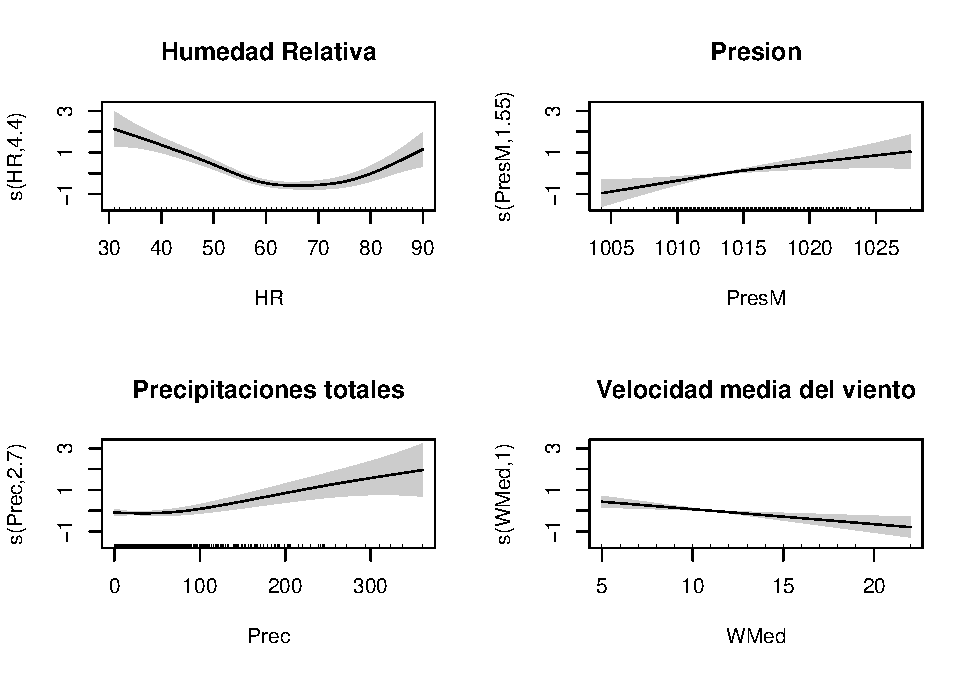
\includegraphics[width=0.95\linewidth]{figurasR/unnamed-chunk-8-1} \end{center}

De las gráficas de la derecha se puede interpretar que los efectos de
\emph{PresM} y \emph{WMed} sobre la temperatura media mensual son
lineales. Ajustamos entonces un nuevo modelo aditivo generalizado del
mismo modo que antes pero imponiendo que el efecto de estas variables
sea lineal:

\begin{Shaded}
\begin{Highlighting}[]
\NormalTok{mag2 }\OtherTok{\textless{}{-}} \FunctionTok{gam}\NormalTok{(TMedM}\SpecialCharTok{\textasciitilde{}} \FunctionTok{s}\NormalTok{(HR)}\SpecialCharTok{+}\NormalTok{PresM}\SpecialCharTok{+}\FunctionTok{s}\NormalTok{(Prec)}\SpecialCharTok{+}\NormalTok{WMed}\SpecialCharTok{+}\NormalTok{Año}\SpecialCharTok{+}\NormalTok{Mes,}\AttributeTok{data =}\NormalTok{ Clima)}
\FunctionTok{summary}\NormalTok{(mag2)}
\end{Highlighting}
\end{Shaded}

\begin{verbatim}
## 
## Family: gaussian 
## Link function: identity 
## 
## Formula:
## TMedM ~ s(HR) + PresM + s(Prec) + WMed + Año + Mes
## 
## Parametric coefficients:
##               Estimate Std. Error t value Pr(>|t|)    
## (Intercept) -1.388e+02  2.690e+01  -5.158 3.22e-07 ***
## PresM        8.417e-02  2.400e-02   3.507 0.000481 ***
## WMed        -7.201e-02  2.235e-02  -3.222 0.001332 ** 
## Año          3.253e-02  2.886e-03  11.272  < 2e-16 ***
## Mes2         1.943e+00  2.315e-01   8.394 2.50e-16 ***
## Mes3         4.559e+00  2.713e-01  16.804  < 2e-16 ***
## Mes4         6.972e+00  3.184e-01  21.899  < 2e-16 ***
## Mes5         1.029e+01  3.402e-01  30.245  < 2e-16 ***
## Mes6         1.391e+01  3.507e-01  39.648  < 2e-16 ***
## Mes7         1.664e+01  3.782e-01  44.011  < 2e-16 ***
## Mes8         1.681e+01  3.730e-01  45.064  < 2e-16 ***
## Mes9         1.420e+01  3.285e-01  43.242  < 2e-16 ***
## Mes10        9.791e+00  2.827e-01  34.635  < 2e-16 ***
## Mes11        4.188e+00  2.366e-01  17.702  < 2e-16 ***
## Mes12        8.095e-01  2.181e-01   3.711 0.000222 ***
## ---
## Signif. codes:  0 '***' 0.001 '**' 0.01 '*' 0.05 '.' 0.1 ' ' 1
## 
## Approximate significance of smooth terms:
##           edf Ref.df      F  p-value    
## s(HR)   4.469  5.551 20.250  < 2e-16 ***
## s(Prec) 2.610  3.294  5.994 0.000342 ***
## ---
## Signif. codes:  0 '***' 0.001 '**' 0.01 '*' 0.05 '.' 0.1 ' ' 1
## 
## R-sq.(adj) =  0.962   Deviance explained = 96.3%
## GCV = 1.4708  Scale est. = 1.4269    n = 740
\end{verbatim}

Podemos ver que tanto la desviación explicada como la estimación del
error por validación cruzada coinciden con las del modelo anterior, sin
embargo utilizaremos la función \emph{anova} para dar una prueba de
razón de verosimilitud que determine si el modelo más complejo mejora
significativamente el ajuste.

\begin{Shaded}
\begin{Highlighting}[]
\FunctionTok{anova}\NormalTok{(mag1,mag2,}\AttributeTok{test =} \StringTok{"F"}\NormalTok{)}
\end{Highlighting}
\end{Shaded}

\begin{verbatim}
## Analysis of Deviance Table
## 
## Model 1: TMedM ~ s(HR) + s(PresM) + s(Prec) + s(WMed) + Año + Mes
## Model 2: TMedM ~ s(HR) + PresM + s(Prec) + WMed + Año + Mes
##   Resid. Df Resid. Dev       Df Deviance      F Pr(>F)
## 1    715.18     1022.3                                
## 2    716.15     1024.4 -0.97706  -2.1327 1.5316 0.2158
\end{verbatim}

Como el p-valor resultante del contraste de hipótesis es \(>0.05\), no
tenemos evidencias significativas como para rechazar la hipótesis nula,
es decir, se acepta que ambos modelos tienen el mismo ajuste.

También es posible compararlos mediante otros criterios, por ejemplo el
AIC (Akaike Information Criterion) que tiene en cuenta el número de
parámetros a estimar y el valor objetivo de la función de
log-verosimilitud:

\begin{Shaded}
\begin{Highlighting}[]
\FunctionTok{AIC}\NormalTok{(mag1,mag2)}
\end{Highlighting}
\end{Shaded}

\begin{verbatim}
##            df      AIC
## mag1 23.65122 2386.466
## mag2 23.07915 2386.864
\end{verbatim}

En este caso son casi idénticos, aunque el primer modelo tiene menor
AIC.

Para obtener más información sobre el modelo planteado se utiliza la
siguiente rutina de diagnósticos que nos proporciona información y
gráficos útiles para evaluar la calidad del ajuste del modelo.

\begin{Shaded}
\begin{Highlighting}[]
\FunctionTok{gam.check}\NormalTok{(mag1)}
\end{Highlighting}
\end{Shaded}

\begin{center}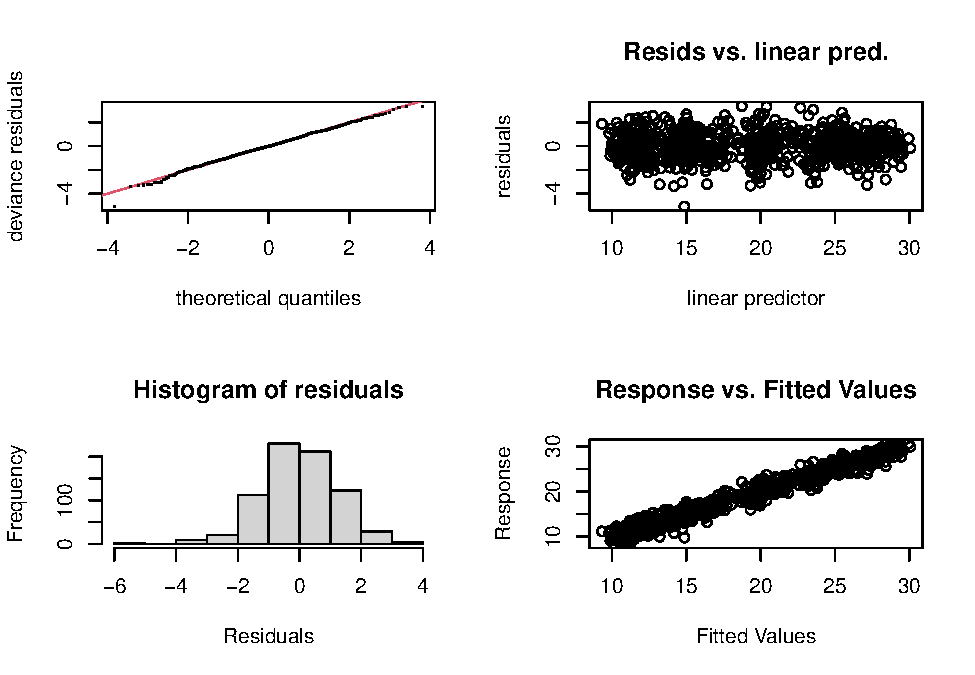
\includegraphics[width=0.95\linewidth]{figurasR/unnamed-chunk-12-1} \end{center}

\begin{verbatim}
## 
## Method: GCV   Optimizer: magic
## Smoothing parameter selection converged after 10 iterations.
## The RMS GCV score gradient at convergence was 1.49324e-07 .
## The Hessian was positive definite.
## Model rank =  49 / 49 
## 
## Basis dimension (k) checking results. Low p-value (k-index<1) may
## indicate that k is too low, especially if edf is close to k'.
## 
##            k'  edf k-index p-value    
## s(HR)    9.00 4.40    0.93   0.020 *  
## s(PresM) 9.00 1.55    0.92   0.010 ** 
## s(Prec)  9.00 2.70    0.94   0.075 .  
## s(WMed)  9.00 1.00    0.87  <2e-16 ***
## ---
## Signif. codes:  0 '***' 0.001 '**' 0.01 '*' 0.05 '.' 0.1 ' ' 1
\end{verbatim}

Por un lado, la salida por consola nos informa de que se obtiene la
convergencia por optimización del GCV y que el modelo es de rango
completo. Los p-valores que aparecen se corresponden a los tests de
residuos aleatorios correspondientes para cada predictor, en este caso
todos excepto el asociado a \emph{Prec} son \(<0.05\), lo que indica que
los residuos no están distribuidos aleatoriamente y que se necesitaría
una base de funciones de mayor dimensión. Por otro lado, observemos qué
representa cada una de las gráficas generadas y cuál sería el caso ideal
para cada una de ellas:

\begin{itemize}
  \item Q-Q Plot: compara la distribución de los residuos con una distribución normal. Lo ideal es que los puntos se alineen aproximadamente en una línea recta.
  \item Resids vs. linear pred: representa los residuos contra el predictor lineal, ayuda a verificar si los residuos se distribuyen aleatoriamente, que sería lo ideal.
  \item Histogram of residuals: se trata de un histograma de los residuos, en este caso lo ideal es que muestre una distribución aproximadamente normal, centrada en cero, esto indicaría que los residuos no presentan sesgos significativos.
  \item Response vs. Fitted Values: representa los valores observados frente a los valores ajustados, lo ideal sería que los puntos resultantes se aconglomerasen en torno a la recta $x=y$.
\end{itemize}

Por lo general este modelo se comporta de manera decente, ya que se
aproxima mucho a los casos ideales de cada gráfica. Podemo utilizar la
librería \emph{visibly} de \citet{M-Clark} para hacer esta
representación de forma más clara:

\begin{Shaded}
\begin{Highlighting}[]
\CommentTok{\#install.packages(\textquotesingle{}visibly\textquotesingle{})}
\FunctionTok{library}\NormalTok{(visibly)}
\FunctionTok{plot\_gam\_check}\NormalTok{(mag1)}
\end{Highlighting}
\end{Shaded}

\begin{center}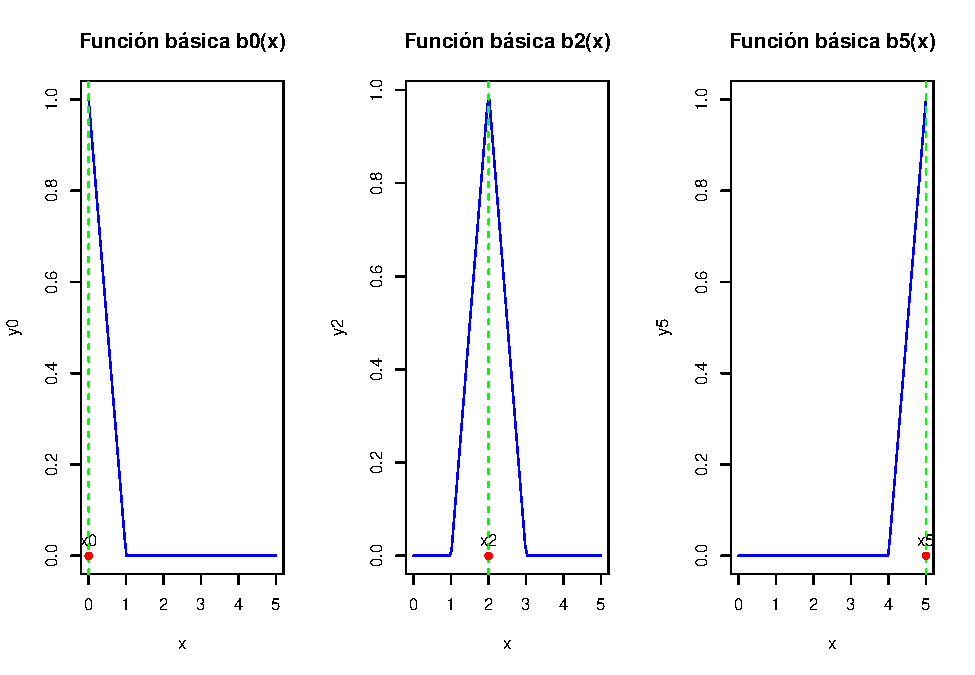
\includegraphics[width=0.95\linewidth]{figurasR/unnamed-chunk-13-1} \end{center}

\hypertarget{visualizaciuxf3n-de-los-resultados}{%
\subsection{Visualización de los
resultados}\label{visualizaciuxf3n-de-los-resultados}}

Una vez generado el modelo y comprobado que se tiene una bondad de
ajuste decente, veamos cómo ajusta los datos para poder visualizar si se
ha producido un cambio significativo en la temperatura media mensual a
lo largo de los años.

\begin{Shaded}
\begin{Highlighting}[]
\NormalTok{Julio }\OtherTok{\textless{}{-}} \FunctionTok{filter}\NormalTok{(Clima, Clima}\SpecialCharTok{$}\NormalTok{Mes }\SpecialCharTok{==} \DecValTok{7}\NormalTok{)}
\NormalTok{Julio}\SpecialCharTok{$}\NormalTok{Preds }\OtherTok{\textless{}{-}} \FunctionTok{predict}\NormalTok{(mag1, }\AttributeTok{newdata =}\NormalTok{ Julio)}
\NormalTok{Julio }\OtherTok{\textless{}{-}}\NormalTok{ Julio[}\FunctionTok{complete.cases}\NormalTok{(Julio}\SpecialCharTok{$}\NormalTok{Preds),]}

\NormalTok{lm1 }\OtherTok{\textless{}{-}} \FunctionTok{gam}\NormalTok{(TMedM }\SpecialCharTok{\textasciitilde{}}\NormalTok{ Año,}\AttributeTok{data =}\NormalTok{ Julio)}
\NormalTok{Julio}\SpecialCharTok{$}\NormalTok{LPreds }\OtherTok{\textless{}{-}} \FunctionTok{predict}\NormalTok{(lm1,Julio)}

\FunctionTok{library}\NormalTok{(ggplot2)}
\FunctionTok{ggplot}\NormalTok{(Julio,}\FunctionTok{aes}\NormalTok{(}\AttributeTok{x=}\NormalTok{Año))}\SpecialCharTok{+}
  \FunctionTok{geom\_point}\NormalTok{(}\FunctionTok{aes}\NormalTok{(}\AttributeTok{y=}\NormalTok{TMedM),}\AttributeTok{size=}\FloatTok{1.5}\NormalTok{, }\AttributeTok{col =} \StringTok{\textquotesingle{}black\textquotesingle{}}\NormalTok{)}\SpecialCharTok{+}
  \FunctionTok{theme\_minimal}\NormalTok{()}\SpecialCharTok{+}
  \FunctionTok{geom\_line}\NormalTok{(}\FunctionTok{aes}\NormalTok{(}\AttributeTok{y=}\NormalTok{Preds, }\AttributeTok{color =} \StringTok{\textquotesingle{}MAG\textquotesingle{}}\NormalTok{),}\AttributeTok{linewidth=}\DecValTok{1}\NormalTok{)}\SpecialCharTok{+}
  \FunctionTok{geom\_line}\NormalTok{(}\FunctionTok{aes}\NormalTok{(}\AttributeTok{y=}\NormalTok{LPreds, }\AttributeTok{color =} \StringTok{\textquotesingle{}ML\textquotesingle{}}\NormalTok{),}\AttributeTok{linewidth=}\FloatTok{0.6}\NormalTok{)}\SpecialCharTok{+}
  \FunctionTok{labs}\NormalTok{(}\AttributeTok{title =}\StringTok{"Temperatura media mensual del mes de Julio"}\NormalTok{,}\AttributeTok{x=}\StringTok{"Año"}\NormalTok{,}\AttributeTok{y=}\StringTok{"Temperatura ºC"}\NormalTok{)}\SpecialCharTok{+}
  \FunctionTok{scale\_color\_manual}\NormalTok{(}\AttributeTok{values =} \FunctionTok{c}\NormalTok{(}\StringTok{\textquotesingle{}MAG\textquotesingle{}} \OtherTok{=} \StringTok{\textquotesingle{}darkred\textquotesingle{}}\NormalTok{, }\StringTok{\textquotesingle{}ML\textquotesingle{}} \OtherTok{=} \StringTok{\textquotesingle{}\#EB6146\textquotesingle{}}\NormalTok{), }\AttributeTok{name =} \StringTok{"Leyenda"}\NormalTok{) }\SpecialCharTok{+} 
  \FunctionTok{theme}\NormalTok{(}\AttributeTok{axis.title =} \FunctionTok{element\_text}\NormalTok{(}\AttributeTok{face =} \StringTok{"bold"}\NormalTok{),}
        \AttributeTok{legend.text =} \FunctionTok{element\_text}\NormalTok{( }\AttributeTok{size =} \DecValTok{10}\NormalTok{,}\AttributeTok{colour =} \StringTok{"black"}\NormalTok{),}
        \AttributeTok{legend.position =} \StringTok{\textquotesingle{}right\textquotesingle{}}\NormalTok{)}
\end{Highlighting}
\end{Shaded}

\begin{center}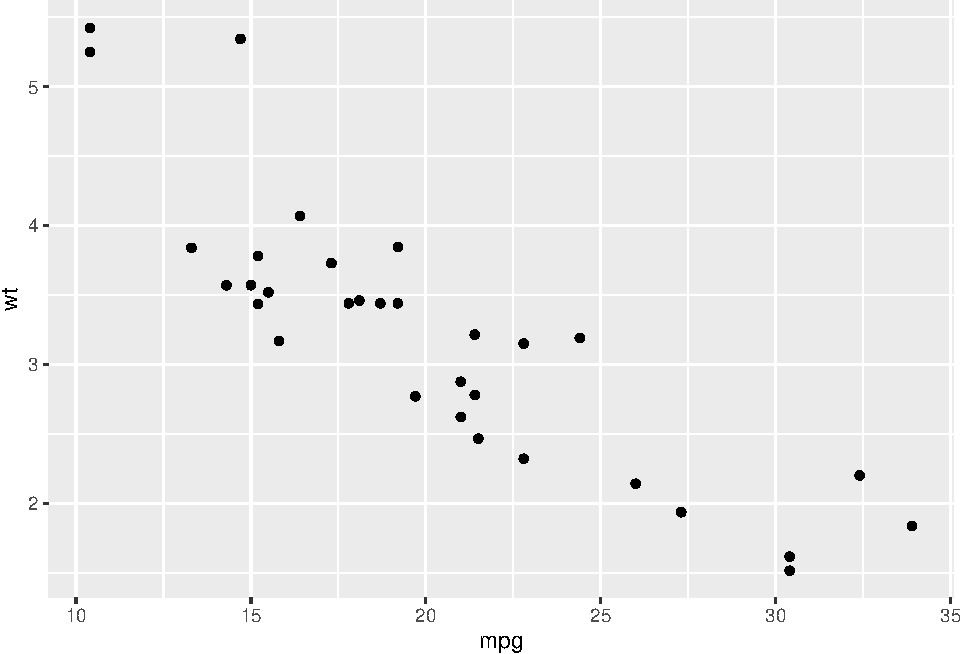
\includegraphics[width=0.95\linewidth]{figurasR/unnamed-chunk-14-1} \end{center}

Con esta gráfica podemos apreciar claramente como la temperatura media
en el mes de Julio ha ido aumentado con el paso de los años en la
estación meteorológica del aeropuerto de San Pablo. Hemos introducido la
recta proporcionada por el modelo lineal para los datos de los meses de
Julio para tener una mejor apreciación de tal incremento.

\hypertarget{modelizaciuxf3n-de-gases-de-efecto-invernadero}{%
\section{Modelización de gases de efecto
invernadero}\label{modelizaciuxf3n-de-gases-de-efecto-invernadero}}

\hypertarget{descripciuxf3n-de-los-datos}{%
\subsection{Descripción de los
datos}\label{descripciuxf3n-de-los-datos}}

En esta sección ajustaremos modelos aditivos generalizados para estudiar
la concentración atmosférica de gases de efecto invernadero, en
particular analizaremos las medias mensuales globales de las
concentraciones de dióxido de carbono (\(CO_2\)), Metano (\(CH_4\)) y
óxido nitroso (\(N_2O\)). Para ello consideraremos los datos
proporcionados por United Nations Environment Programme (UNEP), para el
\(CO_2\) se obtienen en
\url{https://wesr.unep.org/climate/essential-climate-variables-ecv/atmospheric-co2-concentration}
y para los dos siguientes en
\url{https://wesr.unep.org/climate/essential-climate-variables-ecv/atmospheric-ch4-n2o-sf6-concentration}.

Ya hablamos sobre las emisiones de gases contaminantes en
\ref{Resumen del cambio climático en la actualidad} pero no se llego a
definir en qué consistían. Estos gases son capaces de absorber y emitir
radiación dentro del espectro inflarrojo, por tanto son capaces de
retener el calor del Sol, lo que permite que el clima terrestre sea
habitable para la humanidad. Sin embargo, desde el inicio de la
revolución industrial, la actividad humana ha producido un desequilibrio
en los niveles de concentración de estos gases en la atmósfera. En
particular estudiaremos las concentraciones de los tres tipos de gases
antes mencionados por ser los que se emiten en mayor cantidad o por ser
las más potentes (en términos de contribución al efecto invernadero).
Por ejemplo, las emisiones de \(CO_2\) se corresponden aproximadamente
con tres cuartas partes del total de emisiones de GEI, sin embargo el
\(CH_4\) y el \(N_2O\) representan una parte mucho menor que el dióxido
de carbono pero por unidad son mucho más potentes como gases de efecto
invernadero.

Hagamos ahora una primera visualización de los datos. Para tener una
mejor lectura de ellos, primero debemos transformar el archivo a una
hoja de excel \emph{.xlsx}, luego utilizaremos la librería \emph{readxl}
para leerlo y la librería \emph{lubridate} para obtener la fecha como
las variable \emph{Año} y \emph{Mes}:

\begin{Shaded}
\begin{Highlighting}[]
\FunctionTok{library}\NormalTok{(readxl)}
\FunctionTok{library}\NormalTok{(lubridate)}
\end{Highlighting}
\end{Shaded}

\begin{itemize}
\item $CO_2$:
\end{itemize}

\begin{Shaded}
\begin{Highlighting}[]
\NormalTok{CO2 }\OtherTok{\textless{}{-}} \FunctionTok{read\_excel}\NormalTok{(}\StringTok{\textquotesingle{}trends{-}in{-}atmospheric{-}carbon{-}dioxide{-}concentration.xlsx\textquotesingle{}}\NormalTok{)}

\NormalTok{CO2}\SpecialCharTok{$}\NormalTok{DateTime }\OtherTok{\textless{}{-}} \FunctionTok{as.Date}\NormalTok{(CO2}\SpecialCharTok{$}\NormalTok{DateTime) }\CommentTok{\# Creamos las variables año y mes}
\NormalTok{CO2}\SpecialCharTok{$}\NormalTok{Año }\OtherTok{\textless{}{-}} \FunctionTok{as.numeric}\NormalTok{(}\FunctionTok{year}\NormalTok{(CO2}\SpecialCharTok{$}\NormalTok{DateTime))}
\NormalTok{CO2}\SpecialCharTok{$}\NormalTok{Mes }\OtherTok{\textless{}{-}} \FunctionTok{factor}\NormalTok{(}\FunctionTok{month}\NormalTok{(CO2}\SpecialCharTok{$}\NormalTok{DateTime),}\AttributeTok{levels =} \FunctionTok{as.character}\NormalTok{(}\DecValTok{1}\SpecialCharTok{:}\DecValTok{12}\NormalTok{))}
\NormalTok{CO2}\SpecialCharTok{$}\NormalTok{Tmes }\OtherTok{\textless{}{-}} \FunctionTok{as.numeric}\NormalTok{(CO2}\SpecialCharTok{$}\StringTok{\textquotesingle{}Monthly Data\textquotesingle{}}\NormalTok{)}
\NormalTok{CO2}\SpecialCharTok{$}\NormalTok{Trend }\OtherTok{\textless{}{-}} \FunctionTok{as.numeric}\NormalTok{(CO2}\SpecialCharTok{$}\StringTok{\textquotesingle{}Trend\textquotesingle{}}\NormalTok{)}
\NormalTok{CO2 }\OtherTok{\textless{}{-}}\NormalTok{ CO2[,}\FunctionTok{c}\NormalTok{(}\DecValTok{4}\NormalTok{,}\DecValTok{5}\NormalTok{,}\DecValTok{6}\NormalTok{,}\DecValTok{3}\NormalTok{)]}
\NormalTok{CO2 }\OtherTok{\textless{}{-}}\NormalTok{ CO2 }\SpecialCharTok{\%\textgreater{}\%} \FunctionTok{arrange}\NormalTok{(Año, Mes) }
\end{Highlighting}
\end{Shaded}

De este modo nos queda un data frame con 794 observaciones,
correspondientes a los meses desde marzo del 1958 hasta abril de 2024, y
con las variables \emph{Año}, \emph{Mes}, \emph{Tmes} que se corresponde
con la concentración media de \(CO_2\) a nivel global medida en partes
por millón (ppm) y \emph{Trend} que es la media anual de las anteriores.
1 ppm de un gas significa que existe una molécula de ese gas por cada
millón de moléculas de aire.

\begin{Shaded}
\begin{Highlighting}[]
\FunctionTok{str}\NormalTok{(CO2)}
\end{Highlighting}
\end{Shaded}

\begin{verbatim}
## tibble [794 x 4] (S3: tbl_df/tbl/data.frame)
##  $ Año  : num [1:794] 1958 1958 1958 1958 1958 ...
##  $ Mes  : Factor w/ 12 levels "1","2","3","4",..: 3 4 5 6 7 8 9 10 11 12 ...
##  $ Tmes : num [1:794] 316 317 318 317 316 ...
##  $ Trend: num [1:794] NA NA NA NA NA NA NA NA NA NA ...
\end{verbatim}

\begin{Shaded}
\begin{Highlighting}[]
\FunctionTok{summary}\NormalTok{(CO2)}
\end{Highlighting}
\end{Shaded}

\begin{verbatim}
##       Año            Mes           Tmes           Trend      
##  Min.   :1958   3      : 67   Min.   :312.4   Min.   :316.0  
##  1st Qu.:1974   4      : 67   1st Qu.:330.4   1st Qu.:331.1  
##  Median :1991   1      : 66   Median :355.0   Median :355.7  
##  Mean   :1991   2      : 66   Mean   :359.0   Mean   :359.3  
##  3rd Qu.:2007   5      : 66   3rd Qu.:384.6   3rd Qu.:384.0  
##  Max.   :2024   6      : 66   Max.   :426.6   Max.   :421.1  
##                 (Other):396                   NA's   :729
\end{verbatim}

\begin{itemize}
\item $CH_4$:
\end{itemize}

\begin{Shaded}
\begin{Highlighting}[]
\NormalTok{CH4 }\OtherTok{\textless{}{-}} \FunctionTok{read\_excel}\NormalTok{(}\StringTok{\textquotesingle{}trends{-}in{-}atmospheric{-}methane{-}concentration.xlsx\textquotesingle{}}\NormalTok{)}

\NormalTok{CH4}\SpecialCharTok{$}\NormalTok{DateTime }\OtherTok{\textless{}{-}} \FunctionTok{as.Date}\NormalTok{(CH4}\SpecialCharTok{$}\NormalTok{DateTime) }\CommentTok{\# Creamos las variables año y mes }
\NormalTok{CH4}\SpecialCharTok{$}\NormalTok{Año }\OtherTok{\textless{}{-}} \FunctionTok{as.numeric}\NormalTok{(}\FunctionTok{year}\NormalTok{(CH4}\SpecialCharTok{$}\NormalTok{DateTime))}
\NormalTok{CH4}\SpecialCharTok{$}\NormalTok{Mes }\OtherTok{\textless{}{-}} \FunctionTok{factor}\NormalTok{(}\FunctionTok{month}\NormalTok{(CH4}\SpecialCharTok{$}\NormalTok{DateTime),}\AttributeTok{levels =} \FunctionTok{as.character}\NormalTok{(}\DecValTok{1}\SpecialCharTok{:}\DecValTok{12}\NormalTok{))}
\NormalTok{CH4}\SpecialCharTok{$}\NormalTok{Trend }\OtherTok{\textless{}{-}} \FunctionTok{as.numeric}\NormalTok{(CH4}\SpecialCharTok{$}\StringTok{\textquotesingle{}Trend\textquotesingle{}}\NormalTok{)}
\NormalTok{CH4 }\OtherTok{\textless{}{-}}\NormalTok{ CH4[,}\FunctionTok{c}\NormalTok{(}\DecValTok{3}\NormalTok{,}\DecValTok{4}\NormalTok{,}\DecValTok{2}\NormalTok{)]}
\NormalTok{CH4 }\OtherTok{\textless{}{-}}\NormalTok{ CH4 }\SpecialCharTok{\%\textgreater{}\%} \FunctionTok{arrange}\NormalTok{(Año, Mes) }
\end{Highlighting}
\end{Shaded}

En este caso disponemos de 487 observaciones correspondientes a meses
entre 1983 y 2024, las variables de tiempo \emph{Año} y \emph{Mes} y la
variable \emph{Trend} la cual representa la media mensual de
concentración de metano a nivel global medida en partes por billón
(ppb).

\begin{Shaded}
\begin{Highlighting}[]
\FunctionTok{str}\NormalTok{(CH4)}
\end{Highlighting}
\end{Shaded}

\begin{verbatim}
## tibble [487 x 3] (S3: tbl_df/tbl/data.frame)
##  $ Año  : num [1:487] 1983 1983 1983 1983 1983 ...
##  $ Mes  : Factor w/ 12 levels "1","2","3","4",..: 7 8 9 10 11 12 1 2 3 4 ...
##  $ Trend: num [1:487] 1635 1636 1636 1637 1638 ...
\end{verbatim}

\begin{Shaded}
\begin{Highlighting}[]
\FunctionTok{summary}\NormalTok{(CH4)}
\end{Highlighting}
\end{Shaded}

\begin{verbatim}
##       Año            Mes          Trend     
##  Min.   :1983   1      : 41   Min.   :1635  
##  1st Qu.:1993   7      : 41   1st Qu.:1737  
##  Median :2003   8      : 41   Median :1775  
##  Mean   :2003   9      : 41   Mean   :1778  
##  3rd Qu.:2013   10     : 41   3rd Qu.:1816  
##  Max.   :2024   11     : 41   Max.   :1928  
##                 (Other):241
\end{verbatim}

\begin{itemize}
\item $N_2O$:
\end{itemize}

\begin{Shaded}
\begin{Highlighting}[]
\NormalTok{N2O }\OtherTok{\textless{}{-}} \FunctionTok{read\_excel}\NormalTok{(}\StringTok{\textquotesingle{}trends{-}in{-}atmospheric{-}nitrous{-}oxide{-}concentration.xlsx\textquotesingle{}}\NormalTok{)}

\NormalTok{N2O}\SpecialCharTok{$}\NormalTok{DateTime }\OtherTok{\textless{}{-}} \FunctionTok{as.Date}\NormalTok{(N2O}\SpecialCharTok{$}\NormalTok{DateTime) }\CommentTok{\# Creamos las variables año y mes }
\NormalTok{N2O}\SpecialCharTok{$}\NormalTok{Año }\OtherTok{\textless{}{-}} \FunctionTok{as.numeric}\NormalTok{(}\FunctionTok{year}\NormalTok{(N2O}\SpecialCharTok{$}\NormalTok{DateTime))}
\NormalTok{N2O}\SpecialCharTok{$}\NormalTok{Mes }\OtherTok{\textless{}{-}} \FunctionTok{factor}\NormalTok{(}\FunctionTok{month}\NormalTok{(N2O}\SpecialCharTok{$}\NormalTok{DateTime),}\AttributeTok{levels =} \FunctionTok{as.character}\NormalTok{(}\DecValTok{1}\SpecialCharTok{:}\DecValTok{12}\NormalTok{))}
\NormalTok{N2O}\SpecialCharTok{$}\NormalTok{Trend }\OtherTok{\textless{}{-}} \FunctionTok{as.numeric}\NormalTok{(N2O}\SpecialCharTok{$}\StringTok{\textquotesingle{}Trend\textquotesingle{}}\NormalTok{)}
\NormalTok{N2O }\OtherTok{\textless{}{-}}\NormalTok{ N2O[,}\FunctionTok{c}\NormalTok{(}\DecValTok{3}\NormalTok{,}\DecValTok{4}\NormalTok{,}\DecValTok{2}\NormalTok{)]}
\NormalTok{N2O }\OtherTok{\textless{}{-}}\NormalTok{ N2O }\SpecialCharTok{\%\textgreater{}\%} \FunctionTok{arrange}\NormalTok{(Año, Mes) }\CommentTok{\# Ordenamos por año y mes}
\end{Highlighting}
\end{Shaded}

Para el caso del óxido nitroso sólo disponemos datos desde el 2001, por
lo que obtenemos un conjunto de 277 observaciones para las variables
\emph{Año}, \emph{Mes} y \emph{Trend} que representa la media mensual de
concentración de \(N_2O\) a nivel global medida en partes por billón
(ppb).

\begin{Shaded}
\begin{Highlighting}[]
\FunctionTok{str}\NormalTok{(N2O)}
\end{Highlighting}
\end{Shaded}

\begin{verbatim}
## tibble [277 x 3] (S3: tbl_df/tbl/data.frame)
##  $ Año  : num [1:277] 2001 2001 2001 2001 2001 ...
##  $ Mes  : Factor w/ 12 levels "1","2","3","4",..: 1 2 3 4 5 6 7 8 9 10 ...
##  $ Trend: num [1:277] 316 316 316 316 316 ...
\end{verbatim}

\begin{Shaded}
\begin{Highlighting}[]
\FunctionTok{summary}\NormalTok{(N2O)}
\end{Highlighting}
\end{Shaded}

\begin{verbatim}
##       Año            Mes          Trend      
##  Min.   :2001   1      : 24   Min.   :316.0  
##  1st Qu.:2006   2      : 23   1st Qu.:320.0  
##  Median :2012   3      : 23   Median :325.1  
##  Mean   :2012   4      : 23   Mean   :325.6  
##  3rd Qu.:2018   5      : 23   3rd Qu.:330.7  
##  Max.   :2024   6      : 23   Max.   :337.3  
##                 (Other):138
\end{verbatim}

Solo con los resúmenes de los datos para los tres gases, teniendo en
cuenta las medidas en las que vienen dados, ya se puede ver la gran
diferencia que hay entre sus proporciones en la atmósfera.

\hypertarget{descripciuxf3n-de-los-modelos}{%
\subsection{Descripción de los
modelos}\label{descripciuxf3n-de-los-modelos}}

Partiremos definiendo un modelo lineal para los datos de \(CO_2\) que
tenga como variable de respuesta la media mesual global de la
concentración de este gas medida en ppm y como predictoras las variables
\emph{Año} y \emph{Mes}:

\begin{Shaded}
\begin{Highlighting}[]
\NormalTok{magCO2 }\OtherTok{\textless{}{-}} \FunctionTok{gam}\NormalTok{(Tmes }\SpecialCharTok{\textasciitilde{}}\NormalTok{ Año }\SpecialCharTok{+}\NormalTok{ Mes, }\AttributeTok{data =}\NormalTok{ CO2)}
\FunctionTok{summary}\NormalTok{(magCO2)}
\end{Highlighting}
\end{Shaded}

\begin{verbatim}
## 
## Family: gaussian 
## Link function: identity 
## 
## Formula:
## Tmes ~ Año + Mes
## 
## Parametric coefficients:
##               Estimate Std. Error  t value Pr(>|t|)    
## (Intercept) -2.897e+03  1.637e+01 -176.948  < 2e-16 ***
## Año          1.635e+00  8.215e-03  199.022  < 2e-16 ***
## Mes2         7.917e-01  7.697e-01    1.029 0.303997    
## Mes3         1.770e+00  7.668e-01    2.308 0.021232 *  
## Mes4         3.071e+00  7.668e-01    4.004 6.81e-05 ***
## Mes5         3.486e+00  7.697e-01    4.530 6.84e-06 ***
## Mes6         2.925e+00  7.697e-01    3.800 0.000156 ***
## Mes7         1.390e+00  7.697e-01    1.806 0.071250 .  
## Mes8        -6.210e-01  7.697e-01   -0.807 0.420035    
## Mes9        -2.164e+00  7.697e-01   -2.812 0.005046 ** 
## Mes10       -2.111e+00  7.697e-01   -2.743 0.006228 ** 
## Mes11       -7.661e-01  7.697e-01   -0.995 0.319867    
## Mes12        5.563e-01  7.697e-01    0.723 0.470079    
## ---
## Signif. codes:  0 '***' 0.001 '**' 0.01 '*' 0.05 '.' 0.1 ' ' 1
## 
## 
## R-sq.(adj) =   0.98   Deviance explained = 98.1%
## GCV = 19.874  Scale est. = 19.549    n = 794
\end{verbatim}

Podemos observar que representa un 98.1\% de la desviación explicada,
por lo que en principio no parece un mal ajuste, comprobémoslo con el
diagnóstico de residuos como se hizo en el apartado anterior:

\begin{Shaded}
\begin{Highlighting}[]
\FunctionTok{plot\_gam\_check}\NormalTok{(magCO2)}
\end{Highlighting}
\end{Shaded}

\begin{center}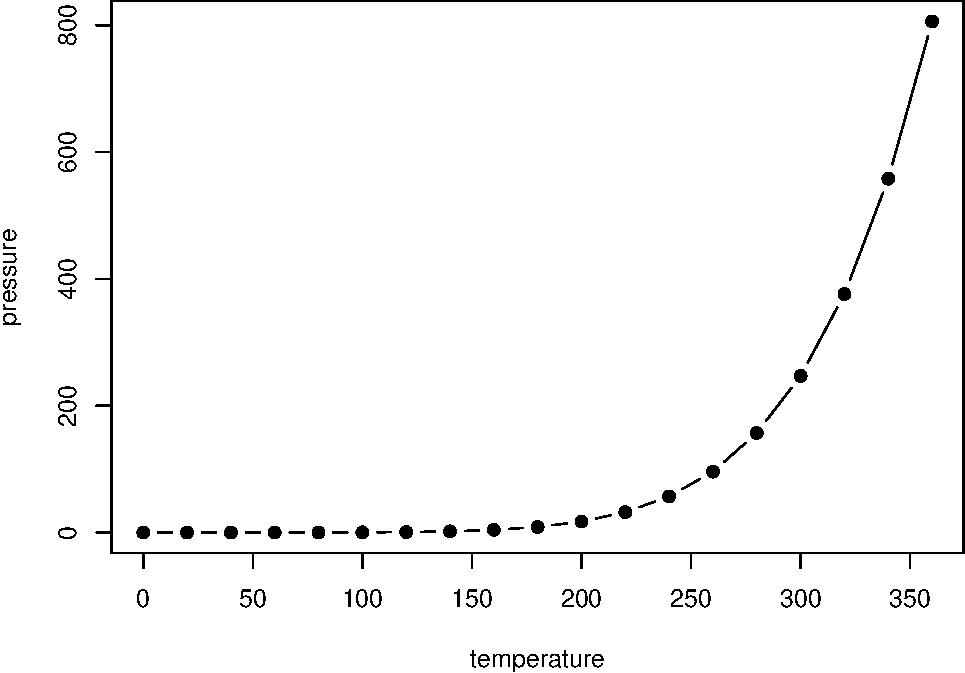
\includegraphics[width=0.95\linewidth]{figurasR/unnamed-chunk-26-1} \end{center}

Gracias a estos gráfios se puede ver cómo el modelo falla en varios
aspectos:

\begin{itemize}
  \item Se puede ver claramente que el Q-Q plot no se adapta a la recta, es decir, la distribución de los residuos no es normal.
  \item En la gráfica de arriba a la derecha se puede ver como los residuos toman un patrón claro respecto de los predictores, lo que implica que la hipótesis de homocedasticidad de los residuos no es cierta.
  \item En la de abajo a la izquierda se ve facilmente no es una distribución normal centrada en el 0, lo que confirma lo observado en el Q-Q plot.
  \item Por último, en el gráfico Response vs. Fitted también se puede intuir la falta de homocedasticidad para los residuos. 
\end{itemize}

Luego, aunque el modelo representanse un gran porcentaje de la
desviación explicada, presenta errores significativos en el análisis de
los residuos por lo que inferimos que el modelo no es adecuado. Para
definir un modelo que se ajuste mejor nos referiremos a dichas gráficas.
En primer lugar, que la gráfica de residuos frente predictores se
asemeje a una función cuadrática nos indica que puede existir una
relación no lineal entre la varible de respuesta y las predictoras, por
lo que será conveniente añadir funciones de suavizado al modelo. Además,
también puede implicar que la familia de distribuciones exponenciales
para la variable de respuesta que estemos utilizando, la normal en este
caso, no sea la adecuada. Podemos utilizar el test de normalidad
univariante Shapiro-Wilk para comprobarlo:

\begin{Shaded}
\begin{Highlighting}[]
\FunctionTok{shapiro.test}\NormalTok{(CO2}\SpecialCharTok{$}\NormalTok{Tmes)}
\end{Highlighting}
\end{Shaded}

\begin{verbatim}
## 
##  Shapiro-Wilk normality test
## 
## data:  CO2$Tmes
## W = 0.9407, p-value < 2.2e-16
\end{verbatim}

Como el p-valor es muy cercano a 0, se rechaza la hipótesis nula de
normalidad de la muestra. Lo que haremos entonces será razonar que como
los datos tratados son niveles de concentraciones positivas, quizás nos
interese utizar la distribución \emph{Gamma} o la \emph{Inverse
Gaussian}. Para determinar cuál de las dos es más conveniente
compararemos los modelos definidos para ambas familias con sus
respectivas funciones de enlace.

\begin{Shaded}
\begin{Highlighting}[]
\NormalTok{magCO2b }\OtherTok{\textless{}{-}} \FunctionTok{gam}\NormalTok{(Tmes }\SpecialCharTok{\textasciitilde{}} \FunctionTok{s}\NormalTok{(Año) }\SpecialCharTok{+}\NormalTok{ Mes, }\AttributeTok{data =}\NormalTok{ CO2, }
               \AttributeTok{family =} \FunctionTok{inverse.gaussian}\NormalTok{(}\AttributeTok{link =} \StringTok{"1/mu\^{}2"}\NormalTok{))}
\FunctionTok{summary}\NormalTok{(magCO2b)}
\end{Highlighting}
\end{Shaded}

\begin{verbatim}
## 
## Family: inverse.gaussian 
## Link function: 1/mu^2 
## 
## Formula:
## Tmes ~ s(Año) + Mes
## 
## Parametric coefficients:
##               Estimate Std. Error  t value Pr(>|t|)    
## (Intercept)  7.962e-06  3.493e-09 2279.492  < 2e-16 ***
## Mes2        -3.316e-08  4.911e-09   -6.754 2.83e-11 ***
## Mes3        -6.782e-08  4.890e-09  -13.869  < 2e-16 ***
## Mes4        -1.217e-07  4.877e-09  -24.956  < 2e-16 ***
## Mes5        -1.462e-07  4.902e-09  -29.820  < 2e-16 ***
## Mes6        -1.229e-07  4.908e-09  -25.040  < 2e-16 ***
## Mes7        -5.866e-08  4.924e-09  -11.913  < 2e-16 ***
## Mes8         2.682e-08  4.945e-09    5.423 7.86e-08 ***
## Mes9         9.343e-08  4.962e-09   18.828  < 2e-16 ***
## Mes10        9.112e-08  4.962e-09   18.364  < 2e-16 ***
## Mes11        3.304e-08  4.947e-09    6.679 4.58e-11 ***
## Mes12       -2.339e-08  4.933e-09   -4.742 2.51e-06 ***
## ---
## Signif. codes:  0 '***' 0.001 '**' 0.01 '*' 0.05 '.' 0.1 ' ' 1
## 
## Approximate significance of smooth terms:
##          edf Ref.df      F p-value    
## s(Año) 8.947  8.999 196755  <2e-16 ***
## ---
## Signif. codes:  0 '***' 0.001 '**' 0.01 '*' 0.05 '.' 0.1 ' ' 1
## 
## R-sq.(adj) =      1   Deviance explained =  100%
## GCV = 9.7546e-09  Scale est. = 9.4978e-09  n = 794
\end{verbatim}

\begin{Shaded}
\begin{Highlighting}[]
\FunctionTok{plot\_gam\_check}\NormalTok{(magCO2b)}
\end{Highlighting}
\end{Shaded}

\begin{center}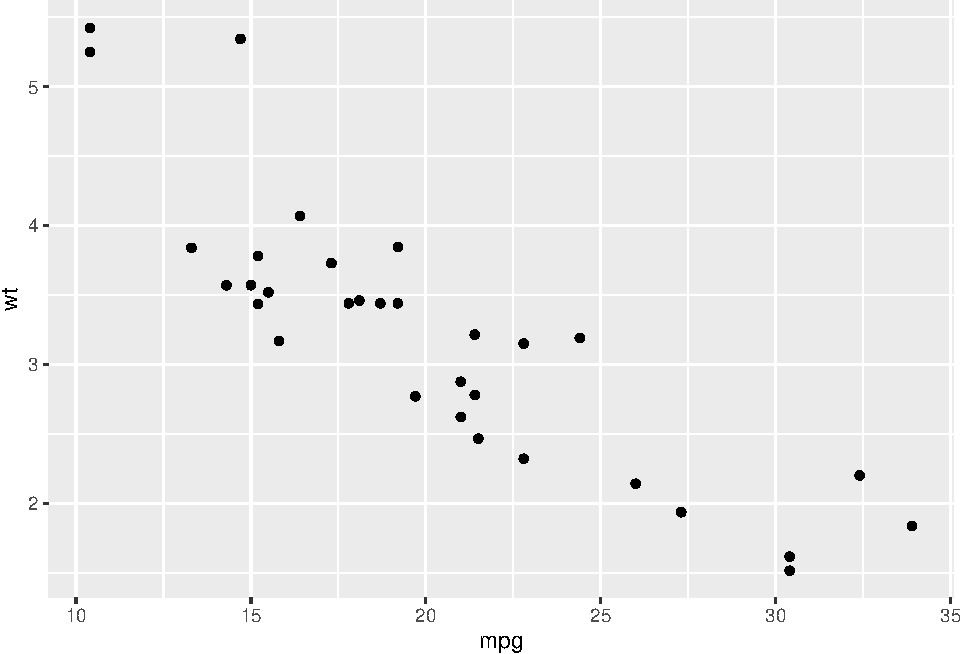
\includegraphics[width=0.95\linewidth]{figurasR/unnamed-chunk-28-1} \end{center}

\begin{Shaded}
\begin{Highlighting}[]
\NormalTok{magCO2c }\OtherTok{\textless{}{-}} \FunctionTok{gam}\NormalTok{(Tmes }\SpecialCharTok{\textasciitilde{}} \FunctionTok{s}\NormalTok{(Año) }\SpecialCharTok{+}\NormalTok{ Mes, }\AttributeTok{data =}\NormalTok{ CO2, }\AttributeTok{family =} \FunctionTok{Gamma}\NormalTok{(}\AttributeTok{link =} \StringTok{"log"}\NormalTok{))}
\FunctionTok{summary}\NormalTok{(magCO2c)}
\end{Highlighting}
\end{Shaded}

\begin{verbatim}
## 
## Family: Gamma 
## Link function: log 
## 
## Formula:
## Tmes ~ s(Año) + Mes
## 
## Parametric coefficients:
##               Estimate Std. Error   t value Pr(>|t|)    
## (Intercept)  5.8777562  0.0001721 34160.995  < 2e-16 ***
## Mes2         0.0021993  0.0002432     9.042  < 2e-16 ***
## Mes3         0.0045205  0.0002424    18.652  < 2e-16 ***
## Mes4         0.0081229  0.0002424    33.516  < 2e-16 ***
## Mes5         0.0097221  0.0002433    39.956  < 2e-16 ***
## Mes6         0.0081689  0.0002433    33.572  < 2e-16 ***
## Mes7         0.0039223  0.0002433    16.120  < 2e-16 ***
## Mes8        -0.0017190  0.0002433    -7.065 3.59e-12 ***
## Mes9        -0.0061035  0.0002433   -25.084  < 2e-16 ***
## Mes10       -0.0059939  0.0002433   -24.634  < 2e-16 ***
## Mes11       -0.0022295  0.0002433    -9.163  < 2e-16 ***
## Mes12        0.0014633  0.0002433     6.014 2.79e-09 ***
## ---
## Signif. codes:  0 '***' 0.001 '**' 0.01 '*' 0.05 '.' 0.1 ' ' 1
## 
## Approximate significance of smooth terms:
##          edf Ref.df      F p-value    
## s(Año) 8.965      9 341186  <2e-16 ***
## ---
## Signif. codes:  0 '***' 0.001 '**' 0.01 '*' 0.05 '.' 0.1 ' ' 1
## 
## R-sq.(adj) =      1   Deviance explained =  100%
## GCV = 2.0052e-06  Scale est. = 1.9524e-06  n = 794
\end{verbatim}

\begin{Shaded}
\begin{Highlighting}[]
\FunctionTok{plot\_gam\_check}\NormalTok{(magCO2c)}
\end{Highlighting}
\end{Shaded}

\begin{center}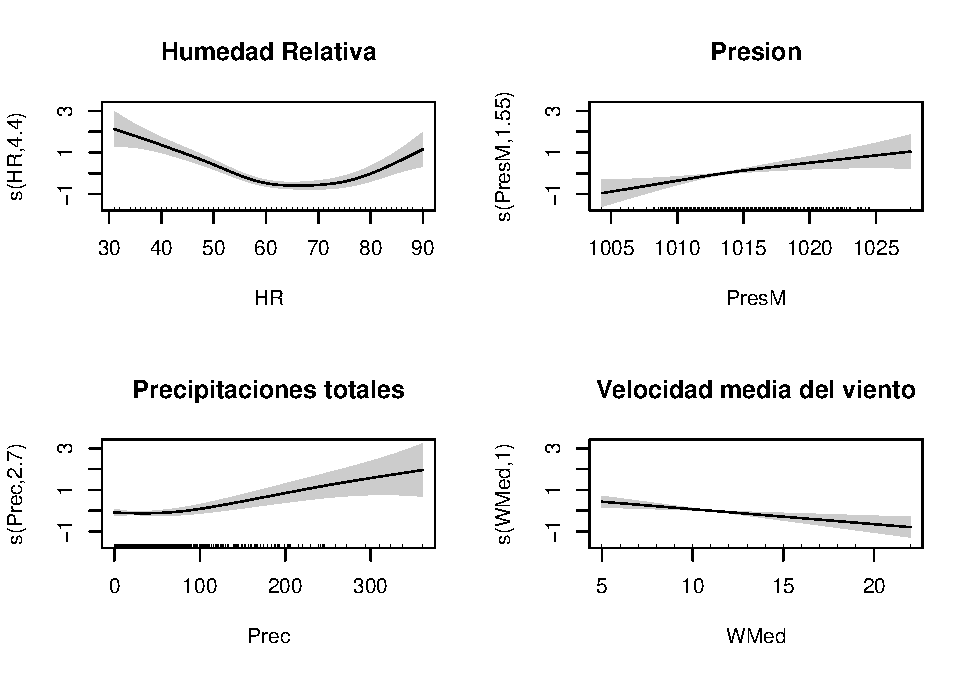
\includegraphics[width=0.95\linewidth]{figurasR/unnamed-chunk-29-1} \end{center}

Vemos ahora como las gráficas para ambos diagnósticos ofrecen resultados
mucho mejores y que incluso los \(R^2_{adj}\) llegan a 1 para los dos
modelos. Comparémoslos:

\begin{verbatim}
##                     AIC          GCV
## Inv. Gauss (b) 1635.459 9.754596e-09
## Gamma (c)      1174.703 2.005172e-06
\end{verbatim}

Por un lado, el modelo c tiene un AIC significativamente menor que el
modelo b. Esto sugiere que el modelo c es mejor en términos de bondad
del ajuste relativo, teniendo en cuenta la penalización de la
complejidad. Por el otro lado, el modelo b tiene un GCV
significativamente menor que el modelo c, por lo que tedrá una mejor
capacidad predictiva y un mejor equilibrio entre ajuste y penalización
por complejidad. Con cuál quedarnos ya dependerá del objetivo que nos
propongamos, para dar un buen ajuste de los datos preferiremos el que
utiliza la familia \emph{Gamma} y para predecir nuevas observaciones
preferiremos el modelo con la familia \emph{Inverse Gaussian}.
Apliquemos estos dos casos:

\hypertarget{visualizaciuxf3n-de-los-resultados-1}{%
\subsection{Visualización de los
resultados}\label{visualizaciuxf3n-de-los-resultados-1}}

\textbf{Ajuste de la concentración del dióxido de carbono} \newline Como
hemos indicado, el MAG que utiliza la distribución \emph{Gamma} como
familia de distribución exponencial proporciona una mejor bondad de
ajuste teniendo en cuenta su complejidad, así que utilizaremos ese para
representar el ajuste de los datos. Se debe tener en cuenta que sobre
las predicciones se debe invertir la función de enlace utilizada, en el
este caso la función logarítmica.

\begin{center}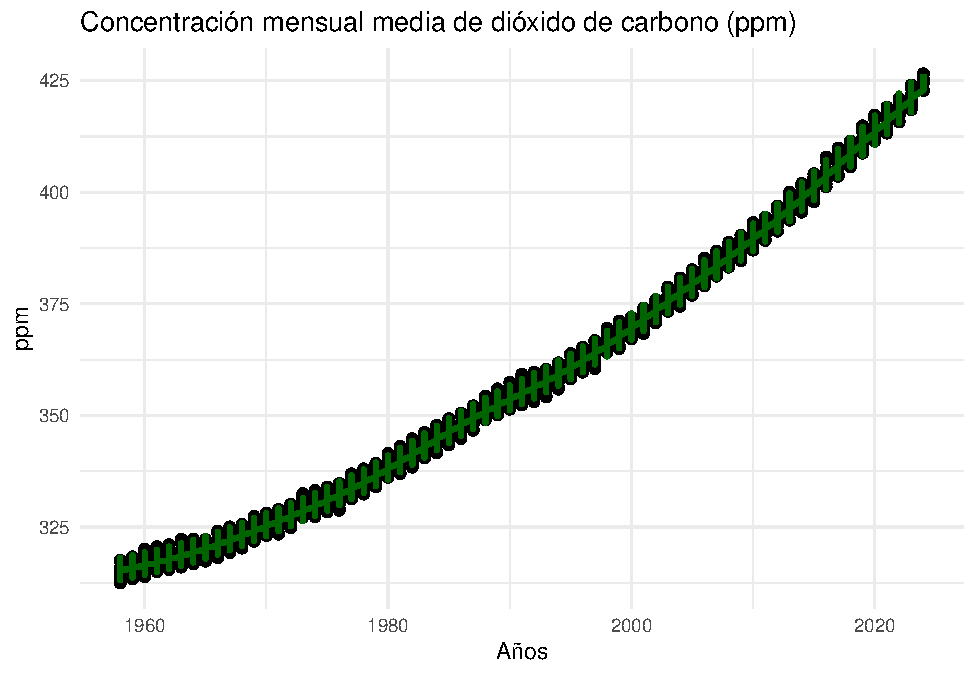
\includegraphics[width=0.95\linewidth]{figurasR/unnamed-chunk-31-1} \end{center}

\textbf{Predicciones de la concentración del dióxido de carbono}
\newline Para representar las predicciones utilizaremos el modelo que
utilizaba la distribución \emph{Inverse Gaussian} pues tenía un menor
valor del error estimado por validación cruzada generalizada.

\begin{center}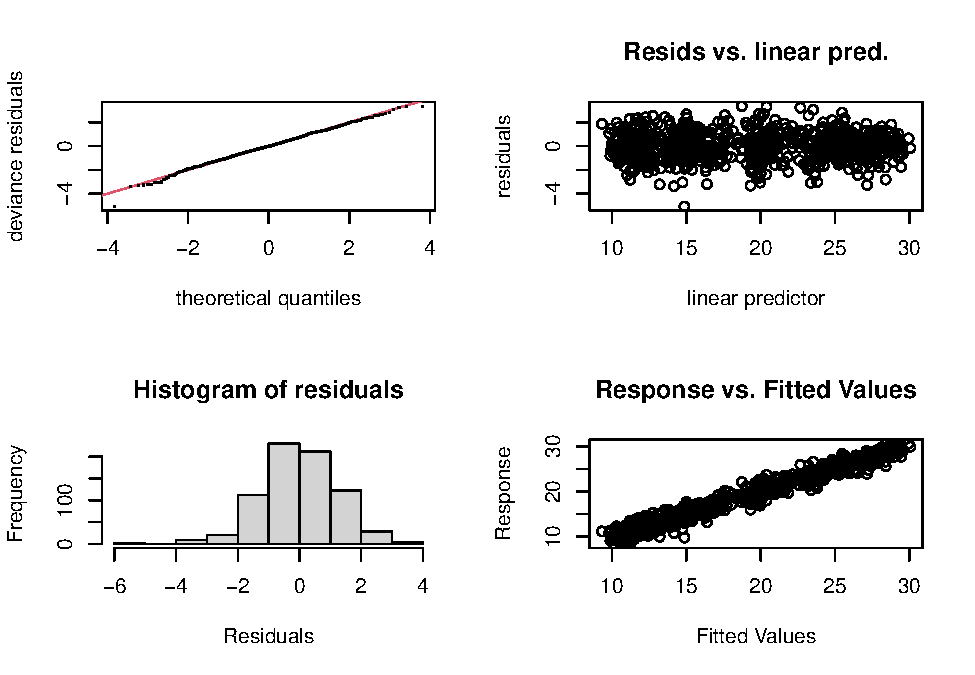
\includegraphics[width=0.95\linewidth]{figurasR/unnamed-chunk-32-1} \end{center}

\begin{verbatim}
## List of 3
##  $ axis.title     :List of 11
##   ..$ family       : NULL
##   ..$ face         : chr "bold"
##   ..$ colour       : NULL
##   ..$ size         : NULL
##   ..$ hjust        : NULL
##   ..$ vjust        : NULL
##   ..$ angle        : NULL
##   ..$ lineheight   : NULL
##   ..$ margin       : NULL
##   ..$ debug        : NULL
##   ..$ inherit.blank: logi FALSE
##   ..- attr(*, "class")= chr [1:2] "element_text" "element"
##  $ legend.text    :List of 11
##   ..$ family       : NULL
##   ..$ face         : NULL
##   ..$ colour       : chr [1:2] "darkgreen" "darkred"
##   ..$ size         : num 10
##   ..$ hjust        : NULL
##   ..$ vjust        : NULL
##   ..$ angle        : NULL
##   ..$ lineheight   : NULL
##   ..$ margin       : NULL
##   ..$ debug        : NULL
##   ..$ inherit.blank: logi FALSE
##   ..- attr(*, "class")= chr [1:2] "element_text" "element"
##  $ legend.position: chr "right"
##  - attr(*, "class")= chr [1:2] "theme" "gg"
##  - attr(*, "complete")= logi FALSE
##  - attr(*, "validate")= logi TRUE
\end{verbatim}

Obviamente esta es una predicción basta que solamente tiene en cuenta el
paso del tiempo y los niveles de concentración medidos hasta ahora. Para
poder hacer predicciones más exactas se necesitarían datos relativos a
las emisiones de \(CO_2\), al clima, al crecimiento de la población y
crecimiento económico y se deberían tener en cuenta políticas sobre
energías, economía y tecnología.

Seguimos el mismo razonamiento para los datos con las concentraciones de
\(CH_4\) y \(N_2O\) para obtener la siguientes representaciones de los
ajustes para cada modelo:

\begin{center}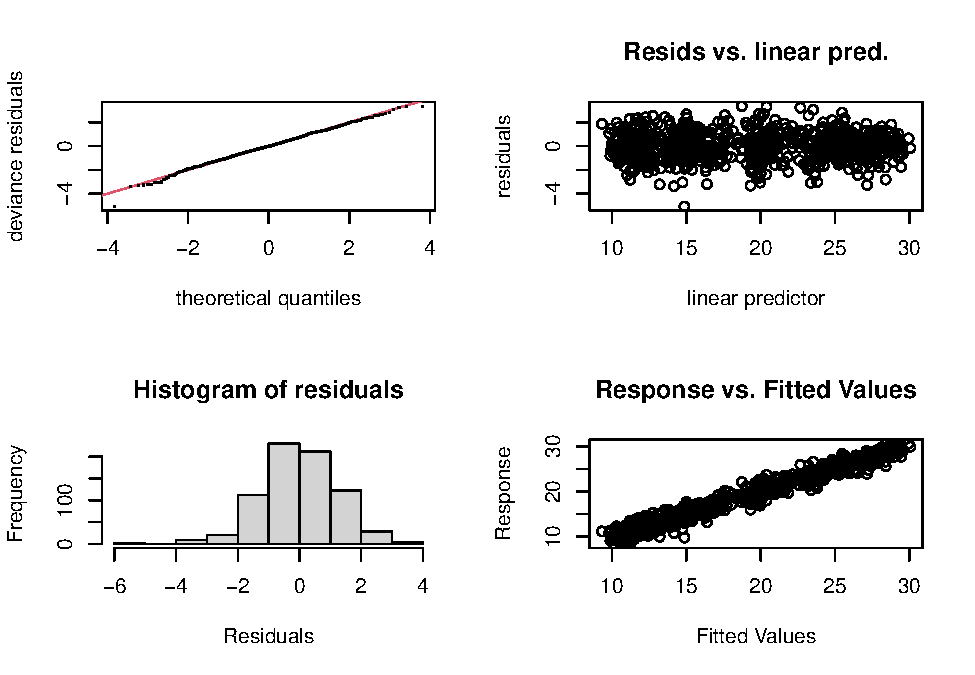
\includegraphics[width=0.95\linewidth]{figurasR/unnamed-chunk-33-1} \end{center}

\begin{center}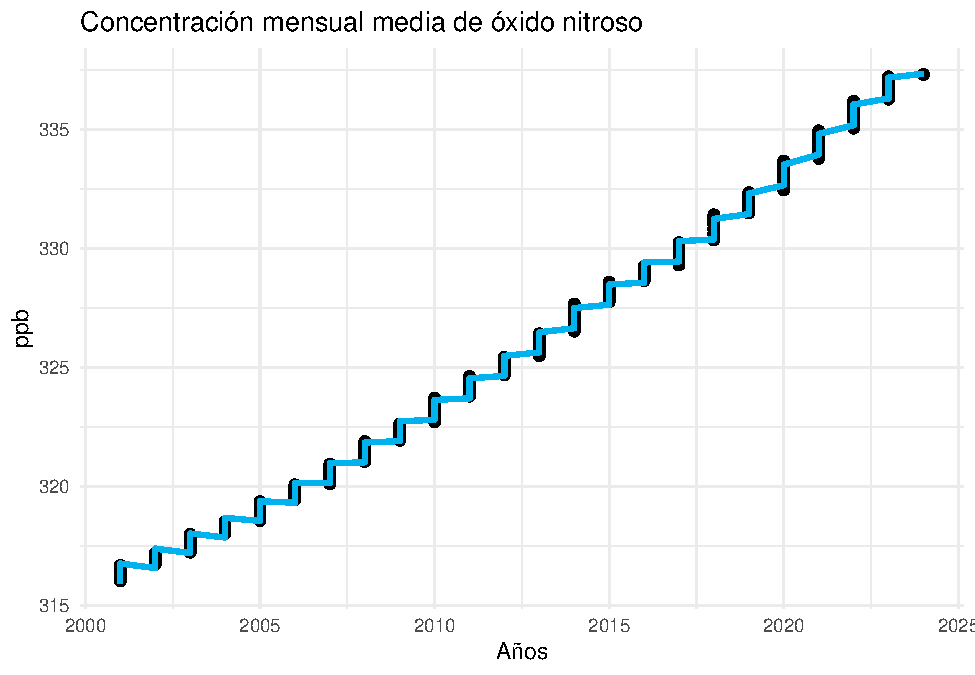
\includegraphics[width=0.95\linewidth]{figurasR/unnamed-chunk-33-2} \end{center}

Se puede apreciar en la primera gráfica que la media mensual de
concentración atmosférica de metano ha aumentado en más de 200 ppb desde
1983 y que la correspondiente al \(N_2O\) ha aumentado en más de 20 ppb
desde el 2001. Comparado con el incremento que se vio anteriormente para
el \(CO_2\) parece poco llamativo, pero como se comentó al principio de
la sección, se debe tener en cuenta que estos dos gases captan mucha mas
radiación que el primero, lo que hace que su aumento, por poco que sea,
también genere preocupación respecto al cambio climático.

\hypertarget{modelizaciuxf3n-del-aumento-del-nivel-del-mar}{%
\section{Modelización del aumento del nivel del
mar}\label{modelizaciuxf3n-del-aumento-del-nivel-del-mar}}

Ya comentamos en la sección
\ref{Resumen del cambio climático en la actualidad} que la subida del
nivel del mar dada en el último siglo es relevante comparada con la de
cualquier siglo anterior. Como se argumenta en \citet{SeaLevelEffects} ,
si este aumento tan pronunciado se progonla a medio-largo plazo pueden
darse grandes consecuencias tales como el incremento de la frecuencia y
la importancia de las inundaciones en zonas costeras, el aumento de
amenazas por fenómenos climáticos extremos como huracanes y grandes
tormentas, la erosión del suelo y las costas que puede implicar la
pérdida del hábitat de peces, pájaros y plantas, etc. Esto conlleva a
que esta sea una de las causas del cambio climático con mayor interés de
estudio. Sin embargo, para poder realizar un análisis aceptable de los
datos asociados a este hecho primero se debe distinguir si se quiere
hacer a nivel global o a nivel local y se necesita disponer de
información relacionada con múltiples factores como: la sanilidad, la
geología del terreno, el deshielo de los polos, las oscilaciones
oceánicas, eventos climáticos extremos que puedan ocurrir o hayan
ocurrido\ldots{}

En nuestro caso no disponemos de tanta información así que nos
proponemos un objetivo más simple como es el definir un modelo aditivo
generalizado que tenga como variable de respuesta la media mensual
global del nivel del mar (GMSL sus siglas en inglés) y como variables
predictoras utilizaremos la media mensual de la temperatura de la
superficie marítima global, la media de concentración atmosférica de
\(CO_2\) (la que utilizamos en la sección anterior como variable
dependiente) y los datos temporales de meses y años.

\hypertarget{descripciuxf3n-de-los-datos-1}{%
\subsection{Descripción de los
datos}\label{descripciuxf3n-de-los-datos-1}}

Como acabamos de comentar, las medidas de concentraciones de \(CO_2\)
que utilizaremos son las mismas que en la sección anterior así que no
entraremos en más detalles para esos datos.

Con respecto a las medidas del GMSL utilizamos la misma fuente de datos
que para los gases de efecto invernadero: la UNEP
\url{https://wesr.unep.org/climate/essential-climate-variables/sea-level-rise},
lo único que debemos tener en cuenta es que se ha modificado el excel de
cierta forma para generar las columnas \emph{Year} y \emph{Month},
correspondientes a la fecha en la que se obtuvo la medición, y la
columna \emph{GMSL} que hasta 1993 se corresponde con las medidas
reconstruidas por la UNEP de la media global del nivel del mar en
milímetros y a partir de ese año es la media de una serie de distintas
medidas satelitales. La carga y limpieza de los datos es la siguiente:

\begin{Shaded}
\begin{Highlighting}[]
\NormalTok{SeaL }\OtherTok{\textless{}{-}} \FunctionTok{read\_excel}\NormalTok{(}\StringTok{\textquotesingle{}SeaLevelv2.xlsx\textquotesingle{}}\NormalTok{)}

\CommentTok{\# Retiramos datos con otro formato y nos quedamos con las variables necesarias.}
\NormalTok{SeaL }\OtherTok{\textless{}{-}}\NormalTok{ SeaL[}\SpecialCharTok{{-}}\NormalTok{(}\DecValTok{1}\SpecialCharTok{:}\DecValTok{240}\NormalTok{),}\FunctionTok{c}\NormalTok{(}\DecValTok{8}\NormalTok{,}\DecValTok{9}\NormalTok{,}\DecValTok{11}\NormalTok{)] }
\CommentTok{\# La variable Año es numérica para la representación como ya se ha indicado otras veces}
\CommentTok{\# y la mensual es categórica}
\NormalTok{SeaL}\SpecialCharTok{$}\NormalTok{Year }\OtherTok{\textless{}{-}} \FunctionTok{as.numeric}\NormalTok{(SeaL}\SpecialCharTok{$}\NormalTok{Year)}
\NormalTok{SeaL}\SpecialCharTok{$}\NormalTok{Month }\OtherTok{\textless{}{-}} \FunctionTok{factor}\NormalTok{(SeaL}\SpecialCharTok{$}\NormalTok{Month,}\AttributeTok{levels =} \DecValTok{1}\SpecialCharTok{:}\DecValTok{12}\NormalTok{)}
\FunctionTok{colnames}\NormalTok{(SeaL) }\OtherTok{\textless{}{-}} \FunctionTok{c}\NormalTok{(}\StringTok{\textquotesingle{}Año\textquotesingle{}}\NormalTok{,}\StringTok{\textquotesingle{}Mes\textquotesingle{}}\NormalTok{,}\StringTok{\textquotesingle{}GMSL\textquotesingle{}}\NormalTok{)}

\CommentTok{\# Como en algunos casos se tienen varias mediciones por mes lo que hacemos es tomar como la }
\CommentTok{\# GMSL mensual la media de todas ellas.}
\NormalTok{SeaL }\OtherTok{\textless{}{-}}\NormalTok{ SeaL }\SpecialCharTok{\%\textgreater{}\%}
  \FunctionTok{group\_by}\NormalTok{(Año, Mes) }\SpecialCharTok{\%\textgreater{}\%}
  \FunctionTok{summarise}\NormalTok{(}\AttributeTok{GMSL =} \FunctionTok{mean}\NormalTok{(GMSL, }\AttributeTok{na.rm =} \ConstantTok{TRUE}\NormalTok{))}
\FunctionTok{summary}\NormalTok{(SeaL)}
\end{Highlighting}
\end{Shaded}

\begin{verbatim}
##       Año            Mes           GMSL        
##  Min.   :1900   1      :123   Min.   :-160.10  
##  1st Qu.:1930   2      :123   1st Qu.:-123.20  
##  Median :1961   3      :123   Median : -67.65  
##  Mean   :1961   4      :123   Mean   : -63.39  
##  3rd Qu.:1992   5      :123   3rd Qu.: -17.02  
##  Max.   :2022   (Other):860   Max.   :  79.31  
##  NA's   :1      NA's   :  1   NA's   :2
\end{verbatim}

Por otro lado, para obtener los datos respectivos a la temperatura media
global nos referiremos a los datos ofrecidos por la NASA en
\url{https://data.giss.nasa.gov/gistemp/}. La preparación de estos datos
para poder ser manejados con comodidad es más compleja y se añade como
un anexo.

\begin{verbatim}
##       Año            Mes             Temp         
##  Min.   :1880   Min.   : 1.00   Min.   :-0.81000  
##  1st Qu.:1916   1st Qu.: 3.75   1st Qu.:-0.22000  
##  Median :1952   Median : 6.50   Median :-0.03000  
##  Mean   :1952   Mean   : 6.50   Mean   : 0.07082  
##  3rd Qu.:1988   3rd Qu.: 9.25   3rd Qu.: 0.29250  
##  Max.   :2024   Max.   :12.00   Max.   : 1.48000  
##  NA's   :12                     NA's   :20
\end{verbatim}

Tras haber cargado los tres conjuntos de datos que necesitaremos para
aplicar el modelo, los unimos en un solo data frame con observaciones
desde 1959 hasta 2015:

\begin{Shaded}
\begin{Highlighting}[]
\NormalTok{SeaL }\OtherTok{\textless{}{-}}\NormalTok{ (SeaL[(}\DecValTok{2015} \SpecialCharTok{\textgreater{}}\NormalTok{ SeaL}\SpecialCharTok{$}\NormalTok{Año) }\SpecialCharTok{\&}\NormalTok{(SeaL}\SpecialCharTok{$}\NormalTok{Año }\SpecialCharTok{\textgreater{}}\DecValTok{1958}\NormalTok{),])[}\DecValTok{1}\SpecialCharTok{:}\DecValTok{672}\NormalTok{,]}
\NormalTok{SeaT }\OtherTok{\textless{}{-}}\NormalTok{ (SeaT[(}\DecValTok{2015} \SpecialCharTok{\textgreater{}}\NormalTok{ SeaT}\SpecialCharTok{$}\NormalTok{Año) }\SpecialCharTok{\&}\NormalTok{ (SeaT}\SpecialCharTok{$}\NormalTok{Año }\SpecialCharTok{\textgreater{}} \DecValTok{1958}\NormalTok{),])[}\DecValTok{1}\SpecialCharTok{:}\DecValTok{672}\NormalTok{,]}
\NormalTok{CO2 }\OtherTok{\textless{}{-}}\NormalTok{  CO2[(}\DecValTok{2015} \SpecialCharTok{\textgreater{}}\NormalTok{ CO2}\SpecialCharTok{$}\NormalTok{Año) }\SpecialCharTok{\&}\NormalTok{ (CO2}\SpecialCharTok{$}\NormalTok{Año }\SpecialCharTok{\textgreater{}} \DecValTok{1958}\NormalTok{),]}

\NormalTok{Sea }\OtherTok{\textless{}{-}} \FunctionTok{cbind}\NormalTok{(SeaL,SeaT,CO2)}
\NormalTok{Sea }\OtherTok{\textless{}{-}}\NormalTok{ Sea[,}\FunctionTok{c}\NormalTok{(}\DecValTok{1}\NormalTok{,}\DecValTok{2}\NormalTok{,}\DecValTok{3}\NormalTok{,}\DecValTok{6}\NormalTok{,}\DecValTok{9}\NormalTok{)]}
\FunctionTok{colnames}\NormalTok{(Sea) }\OtherTok{\textless{}{-}} \FunctionTok{c}\NormalTok{(}\StringTok{\textquotesingle{}Año\textquotesingle{}}\NormalTok{,}\StringTok{\textquotesingle{}Mes\textquotesingle{}}\NormalTok{,}\StringTok{\textquotesingle{}GMSL\textquotesingle{}}\NormalTok{,}\StringTok{\textquotesingle{}Temp\textquotesingle{}}\NormalTok{,}\StringTok{\textquotesingle{}CO2\textquotesingle{}}\NormalTok{)}
\FunctionTok{str}\NormalTok{(Sea)}
\end{Highlighting}
\end{Shaded}

\begin{verbatim}
## tibble [672 x 5] (S3: tbl_df/tbl/data.frame)
##  $ Año : num [1:672] 1959 1959 1959 1959 1959 ...
##  $ Mes : Factor w/ 12 levels "1","2","3","4",..: 1 2 3 4 5 6 7 8 9 10 ...
##  $ GMSL: num [1:672] -65.4 -68.7 -70.8 -70.1 -69.7 -68.3 -68 -65.6 -66.6 -65 ...
##  $ Temp: num [1:672] 0.08 0.07 0.18 0.16 0.04 0.03 0.03 -0.01 -0.06 -0.07 ...
##  $ CO2 : num [1:672] 316 316 317 318 318 ...
\end{verbatim}

\begin{Shaded}
\begin{Highlighting}[]
\FunctionTok{summary}\NormalTok{(Sea)}
\end{Highlighting}
\end{Shaded}

\begin{verbatim}
##       Año            Mes           GMSL              Temp        
##  Min.   :1959   1      : 56   Min.   :-80.700   Min.   :-0.3500  
##  1st Qu.:1973   2      : 56   1st Qu.:-48.675   1st Qu.: 0.0400  
##  Median :1986   3      : 56   Median :-24.250   Median : 0.2650  
##  Mean   :1986   4      : 56   Mean   :-22.486   Mean   : 0.2803  
##  3rd Qu.:2000   5      : 56   3rd Qu.:  1.978   3rd Qu.: 0.5200  
##  Max.   :2014   6      : 56   Max.   : 47.987   Max.   : 1.0200  
##                 (Other):336                                      
##       CO2       
##  Min.   :313.3  
##  1st Qu.:328.3  
##  Median :348.7  
##  Mean   :350.9  
##  3rd Qu.:370.8  
##  Max.   :402.0  
## 
\end{verbatim}

\hypertarget{descripciuxf3n-del-modelo-1}{%
\subsection{Descripción del modelo}\label{descripciuxf3n-del-modelo-1}}

Procedemos de forma similar a las secciones anteriores:

\begin{Shaded}
\begin{Highlighting}[]
\NormalTok{magSL }\OtherTok{\textless{}{-}} \FunctionTok{gam}\NormalTok{(GMSL }\SpecialCharTok{\textasciitilde{}} \FunctionTok{s}\NormalTok{(Temp) }\SpecialCharTok{+} \FunctionTok{s}\NormalTok{(CO2) }\SpecialCharTok{+} \FunctionTok{s}\NormalTok{(Año) }\SpecialCharTok{+}\NormalTok{ Mes, }\AttributeTok{data =}\NormalTok{ Sea) }
\FunctionTok{summary}\NormalTok{(magSL)}
\end{Highlighting}
\end{Shaded}

\begin{verbatim}
## 
## Family: gaussian 
## Link function: identity 
## 
## Formula:
## GMSL ~ s(Temp) + s(CO2) + s(Año) + Mes
## 
## Parametric coefficients:
##             Estimate Std. Error t value Pr(>|t|)    
## (Intercept) -22.9481     0.6614 -34.695  < 2e-16 ***
## Mes2         -0.6542     0.9125  -0.717 0.473643    
## Mes3         -1.6037     1.0743  -1.493 0.135988    
## Mes4         -2.0515     1.4304  -1.434 0.152006    
## Mes5         -2.3487     1.6201  -1.450 0.147629    
## Mes6         -1.7603     1.4375  -1.225 0.221208    
## Mes7         -0.9714     1.0356  -0.938 0.348583    
## Mes8          0.8961     0.8931   1.003 0.316067    
## Mes9          2.9220     1.2168   2.401 0.016616 *  
## Mes10         4.0794     1.2121   3.366 0.000809 ***
## Mes11         3.9769     0.9256   4.297    2e-05 ***
## Mes12         3.0620     0.8820   3.472 0.000552 ***
## ---
## Signif. codes:  0 '***' 0.001 '**' 0.01 '*' 0.05 '.' 0.1 ' ' 1
## 
## Approximate significance of smooth terms:
##           edf Ref.df      F p-value    
## s(Temp) 1.000  1.000  8.967 0.00285 ** 
## s(CO2)  8.083  8.768 10.085 < 2e-16 ***
## s(Año)  8.279  8.820 18.497 < 2e-16 ***
## ---
## Signif. codes:  0 '***' 0.001 '**' 0.01 '*' 0.05 '.' 0.1 ' ' 1
## 
## R-sq.(adj) =   0.98   Deviance explained = 98.1%
## GCV = 21.716  Scale est. = 20.768    n = 672
\end{verbatim}

La desviación explicada por el modelo es del 98.1\% y el error estimado
por validación cruzada generalizada es de 21.716.

\begin{center}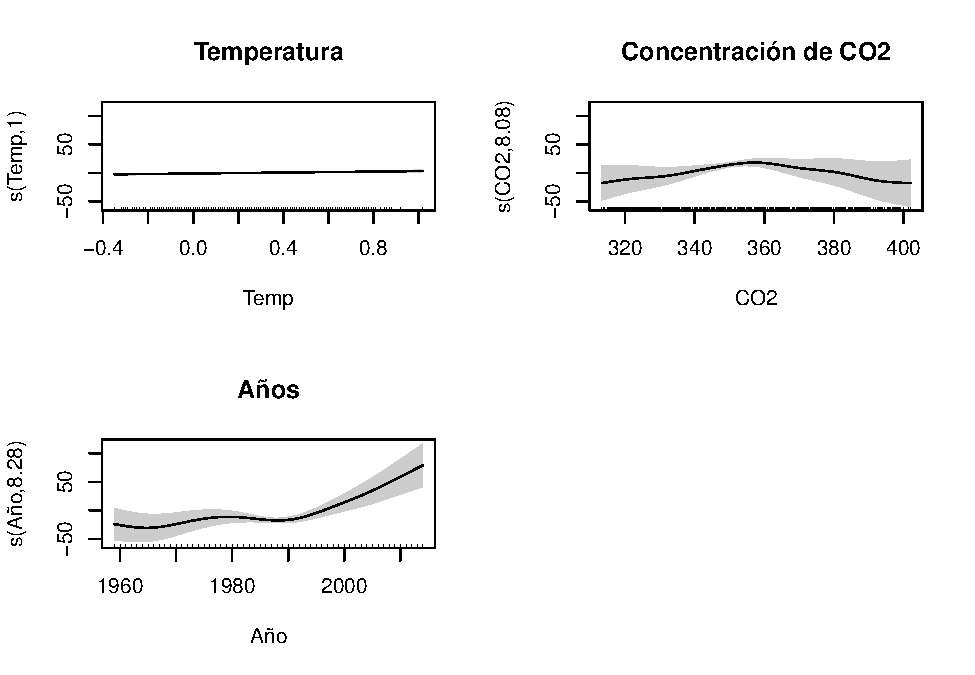
\includegraphics[width=0.95\linewidth]{figurasR/unnamed-chunk-38-1} \end{center}

Hay indicios de que la relación de la variable \emph{Temp} tenga un
efecto lineal sobre la variable de respuesta. Lo comprobamos como
hicimos en \ref{Modelización de la temperatura media mensual}.

\begin{verbatim}
## Analysis of Deviance Table
## 
## Model 1: GMSL ~ s(Temp) + s(CO2) + s(Año) + Mes
## Model 2: GMSL ~ Temp + s(CO2) + s(Año) + Mes
##   Resid. Df Resid. Dev          Df   Deviance      F    Pr(>F)    
## 1    641.41      13346                                            
## 2    641.41      13346 -1.7322e-05 -0.0016203 4.5043 8.293e-05 ***
## ---
## Signif. codes:  0 '***' 0.001 '**' 0.01 '*' 0.05 '.' 0.1 ' ' 1
\end{verbatim}

En este caso como el p-valor es cercano a 0 se rechaza la hipótesis
nula, por lo que se trata de modelos distintos. Por comodidad
trabajaremos con el primero, partimos estudiando las gráficas de
diagnóstico:

\begin{center}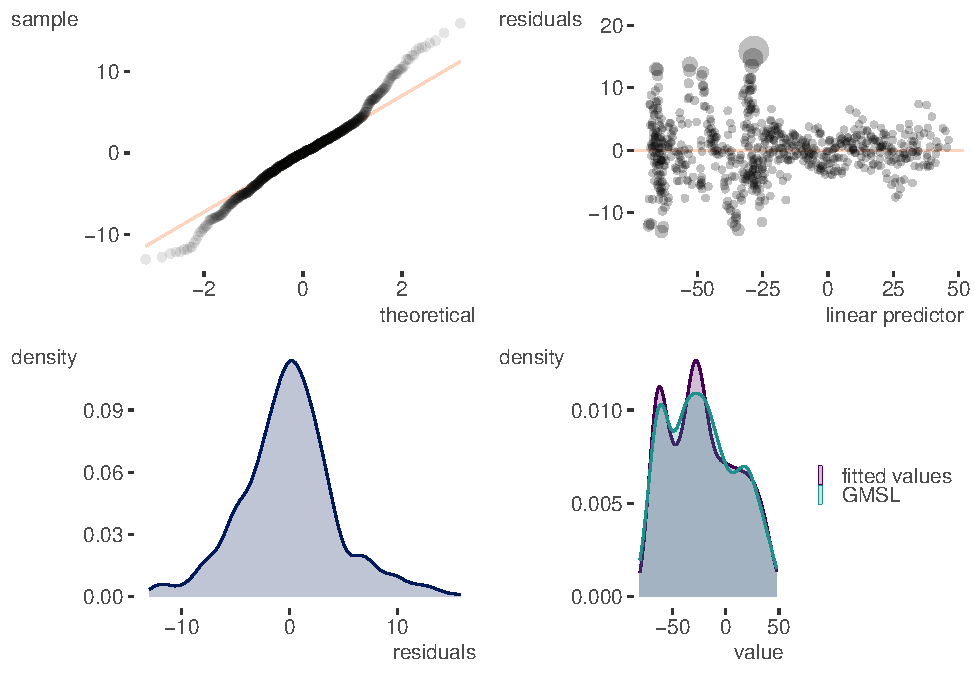
\includegraphics[width=0.95\linewidth]{figurasR/unnamed-chunk-40-1} \end{center}

En este caso nos encontramos principalmente frente a dos problemas. Por
una parte, en la gráfica Q-Q plot podemos observar que en los extremos
los puntos no se ajustan correctamente a la recta, se puede interpretar
que se tienen colas más pesadas, es decir, los valores extremos se
alejan de seguir una distribución normal. Por otra parte, en la gráfica
de arriba a la derecha se puede intuir un patrón en los residuos, lo que
sugiere que no se verifique la hipótesis de varianza constante.

Representemos los datos ajustados por el modelo:

\begin{Shaded}
\begin{Highlighting}[]
\NormalTok{Julio }\OtherTok{\textless{}{-}}\NormalTok{ Sea[Sea}\SpecialCharTok{$}\NormalTok{Mes }\SpecialCharTok{==} \DecValTok{7}\NormalTok{,]}
\NormalTok{Julio}\SpecialCharTok{$}\NormalTok{preds }\OtherTok{\textless{}{-}} \FunctionTok{predict}\NormalTok{(magSL, }\AttributeTok{newdata =}\NormalTok{ Julio)}

\FunctionTok{ggplot}\NormalTok{(}\AttributeTok{data =}\NormalTok{ Julio, }\FunctionTok{aes}\NormalTok{(}\AttributeTok{x =}\NormalTok{ Año, }\AttributeTok{y =}\NormalTok{ GMSL)) }\SpecialCharTok{+}
  \FunctionTok{geom\_point}\NormalTok{() }\SpecialCharTok{+}
  \FunctionTok{geom\_line}\NormalTok{(}\FunctionTok{aes}\NormalTok{(}\AttributeTok{x =}\NormalTok{ Año, }\AttributeTok{y =}\NormalTok{ preds), }\AttributeTok{color =} \StringTok{"darkblue"}\NormalTok{, }\AttributeTok{linewidth =} \DecValTok{1}\NormalTok{) }\SpecialCharTok{+}
  \FunctionTok{labs}\NormalTok{(}\AttributeTok{x =} \StringTok{"Años"}\NormalTok{, }\AttributeTok{y =} \StringTok{"Media Global del nivel del mar"}\NormalTok{, }
       \AttributeTok{title =} \StringTok{"MAG de la media global del nivel del mar"}\NormalTok{) }\SpecialCharTok{+}
  \FunctionTok{theme\_minimal}\NormalTok{()}
\end{Highlighting}
\end{Shaded}

\begin{center}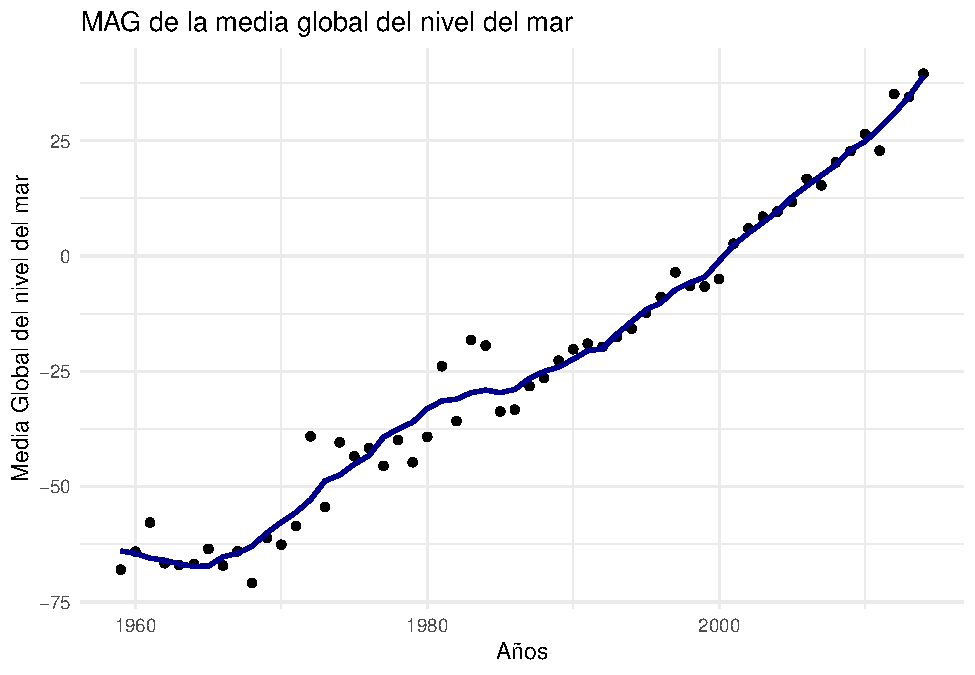
\includegraphics[width=0.95\linewidth]{figurasR/unnamed-chunk-41-1} \end{center}

Es preferible ver cómo varía el nivel del mar fijando un mes que
representando todos los datos a la vez pues entonces se tiene el ruido
de las variaciones entre estaciones.

\begin{center}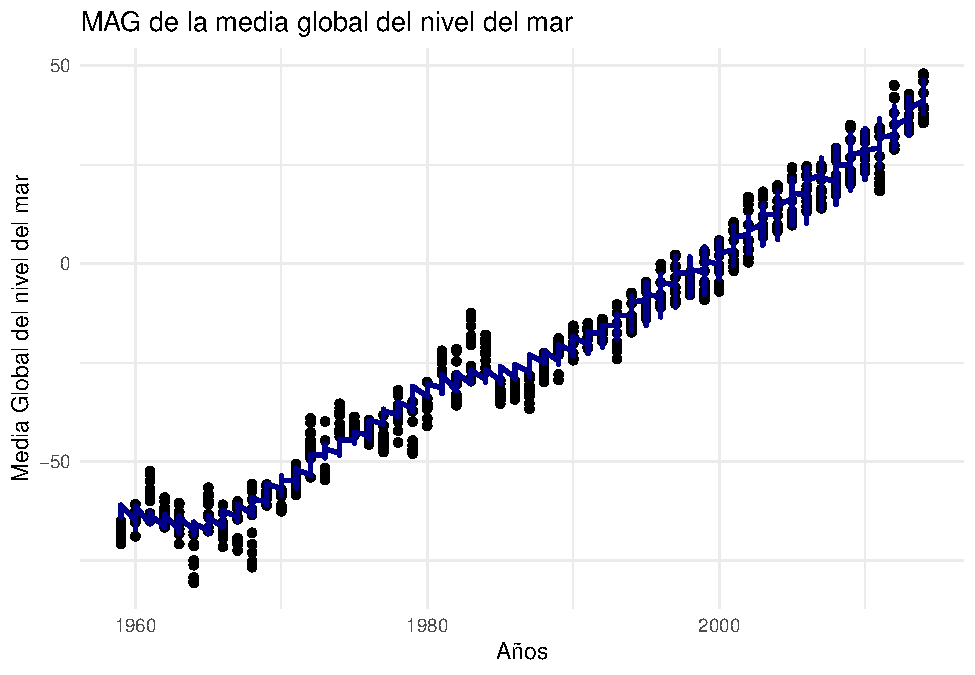
\includegraphics[width=0.95\linewidth]{figurasR/unnamed-chunk-42-1} \end{center}

\bibliography{bib/library.bib,bib/paquetes.bib}


\addcontentsline{toc}{chapter}{Bibliografía}


\end{document}
